\documentclass[12pt, twoside, openright]{report} %fuente a 12pt, formato doble pagina y chapter a la derecha
\raggedbottom % No ajustar el contenido con un salto de pagina

% MÁRGENES: 2,5 cm sup. e inf.; 3 cm izdo. y dcho.
\usepackage[
a4paper,
vmargin=2.5cm,
hmargin=3cm
]{geometry}

% INTERLINEADO: Estrecho (6 ptos./interlineado 1,15) o Moderado (6 ptos./interlineado 1,5)
\renewcommand{\baselinestretch}{1.15}
\parskip=6pt

% DEFINICIÓN DE COLORES para portada y listados de código
\usepackage[table]{xcolor}
\definecolor{azulUC3M}{RGB}{0,0,102}
\definecolor{gray97}{gray}{.97}
\definecolor{gray75}{gray}{.75}
\definecolor{gray45}{gray}{.45}

% Soporte para GENERAR PDF/A
\usepackage[a-1b]{pdfx}

% ENLACES
\usepackage{hyperref}
\hypersetup{colorlinks=true,
	linkcolor=black, % enlaces a partes del documento (p.e. índice) en color negro
	urlcolor=blue} % enlaces a recursos fuera del documento en azul

% Añadir pdfs como partes del documento
\usepackage{pdfpages}

% Quitar la indentación de principio de los parrafos
\setlength{\parindent}{0em}

% EXPRESIONES MATEMATICAS
\usepackage{amsmath,amssymb,amsfonts,amsthm}

\usepackage{txfonts} 
\usepackage[T1]{fontenc}
\usepackage[utf8]{inputenc}

% Insertar graficas y fotos
\usepackage{tikz}
\usepackage{pgfplots}

\usepackage[spanish, es-tabla]{babel} 
\usepackage[babel, spanish=spanish]{csquotes}
\AtBeginEnvironment{quote}{\small}

% diseño de PIE DE PÁGINA
\usepackage{fancyhdr}
\pagestyle{fancy}
\fancyhf{}
\renewcommand{\headrulewidth}{0pt}
\fancyfoot[LE,RO]{\thepage}
\fancypagestyle{plain}{\pagestyle{fancy}}

% DISEÑO DE LOS TÍTULOS de las partes del trabajo (capítulos y epígrafes o subcapítulos)
\usepackage{titlesec}
\usepackage{titletoc}
\titleformat{\chapter}[block]
{\large\bfseries\filcenter}
{\thechapter.}
{5pt}
{\MakeUppercase}
{}
\titlespacing{\chapter}{0pt}{0pt}{*3}
\titlecontents{chapter}
[0pt]                                               
{}
{\contentsmargin{0pt}\thecontentslabel.\enspace\uppercase}
{\contentsmargin{0pt}\uppercase}                        
{\titlerule*[.7pc]{.}\contentspage}                 

\titleformat{\section}
{\bfseries}
{\thesection.}
{5pt}
{}
\titlecontents{section}
[5pt]                                               
{}
{\contentsmargin{0pt}\thecontentslabel.\enspace}
{\contentsmargin{0pt}}
{\titlerule*[.7pc]{.}\contentspage}

\titleformat{\subsection}
{\normalsize\bfseries}
{\thesubsection.}
{5pt}
{}
\titlecontents{subsection}
[10pt]                                               
{}
{\contentsmargin{0pt}                          
	\thecontentslabel.\enspace}
{\contentsmargin{0pt}}                        
{\titlerule*[.7pc]{.}\contentspage}  


% DISEÑO DE TABLAS.
\usepackage{multirow} % permite combinar celdas 
\usepackage{caption} % para personalizar el título de tablas y figuras
\usepackage{floatrow} % utilizamos este paquete y sus macros \ttabbox y \ffigbox para alinear los nombres de tablas y figuras de acuerdo con el estilo definido. Para su uso ver archivo de ejemplo 
\usepackage{array} % con este paquete podemos definir en la siguiente línea un nuevo tipo de columna para tablas: ancho personalizado y contenido centrado
\newcolumntype{P}[1]{>{\centering\arraybackslash}p{#1}}
\DeclareCaptionFormat{upper}{#1#2\uppercase{#3}\par}

% Diseño de tabla para ingeniería
\captionsetup[table]{
	format=hang,
	name=Tabla,
	justification=centering,
	labelsep=colon,
	width=.75\linewidth,
	labelfont=small,
	font=small,
}

% DISEÑO DE FIGURAS.
\usepackage{graphicx}
\graphicspath{{img/}} %ruta a la carpeta de imágenes

% Diseño de figuras para ingeniería
\captionsetup[figure]{
	format=hang,
	name=Fig.,
	singlelinecheck=off,
	labelsep=colon,
	labelfont=small,
	font=small		
}

% NOTAS A PIE DE PÁGINA
\usepackage{chngcntr} %para numeración continua de las notas al pie
\counterwithout{footnote}{chapter}

% LISTADOS DE CÓDIGO
% soporte y estilo para listados de código. Más información en https://es.wikibooks.org/wiki/Manual_de_LaTeX/Listados_de_código/Listados_con_listings
\usepackage{listings}

% definimos un estilo de listings
\lstdefinestyle{estilo}{ frame=Ltb,
	framerule=0pt,
	aboveskip=0.5cm,
	framextopmargin=3pt,
	framexbottommargin=3pt,
	framexleftmargin=0.4cm,
	framesep=0pt,
	rulesep=.4pt,
	backgroundcolor=\color{gray97},
	rulesepcolor=\color{black},
	%
	basicstyle=\ttfamily\footnotesize,
	keywordstyle=\bfseries,
	stringstyle=\ttfamily,
	showstringspaces = false,
	commentstyle=\color{gray45},     
	%
	numbers=left,
	numbersep=15pt,
	numberstyle=\tiny,
	numberfirstline = false,
	breaklines=true,
	xleftmargin=\parindent
}

\captionsetup[lstlisting]{font=small, labelsep=period}
% fijamos el estilo a utilizar 
\lstset{style=estilo}
\renewcommand{\lstlistingname}{\uppercase{Código}}

\pgfplotsset{compat=1.17} 
%-------------
%	DOCUMENTO
%-------------

\begin{document}
\pagenumbering{roman} % Se utilizan cifras romanas en la numeración de las páginas previas al cuerpo del trabajo
	
%----------
%	PORTADA
%----------	
\begin{titlepage}
	\begin{sffamily}
	\color{azulUC3M}
	\begin{center}
		\begin{figure}[H] %incluimos el logotipo de la Universidad
			\makebox[\textwidth][c]{
\includegraphics[width=16cm]{Portada_Logo.png}}
		\end{figure}
		\vspace{2.5cm}
		\begin{Large}
			Grado en Ingeniería Informática\\			
			2019-2020\\
			\vspace{2cm}		
			\textsl{Apuntes}\\
			\bigskip
		\end{Large}
		 	{\Huge Sistemas Operativos}\\
		 	\vspace*{0.5cm}
	 		\rule{10.5cm}{0.1mm}\\
			\vspace*{0.9cm}
			{\LARGE Jorge Rodríguez Fraile\footnote{\href{mailto:100405951@alumnos.uc3m.es}{Universidad: 100405951@alumnos.uc3m.es}  |  \href{mailto:jrf1616@gmail.com}{Personal: jrf1616@gmail.com}}}\\ 
			\vspace*{1cm}
	\end{center}
	\vfill
	\color{black}
		
\includegraphics[width=4.2cm]{img/creativecommons.png}\\
		Esta obra se encuentra sujeta a la licencia Creative Commons\\ \textbf{Reconocimiento - No Comercial - Sin Obra Derivada}
	\end{sffamily}
\end{titlepage}

%----------
%	ÍNDICES
%----------	

%--
% Índice general
%-
\tableofcontents
\thispagestyle{fancy}

%----------
%	TRABAJO
%----------	
\pagenumbering{arabic} % numeración con múmeros arábigos para el resto de la publicación	


%----------
%	COMENZAR A ESCRIBIR AQUI
%----------	


\part{Información}
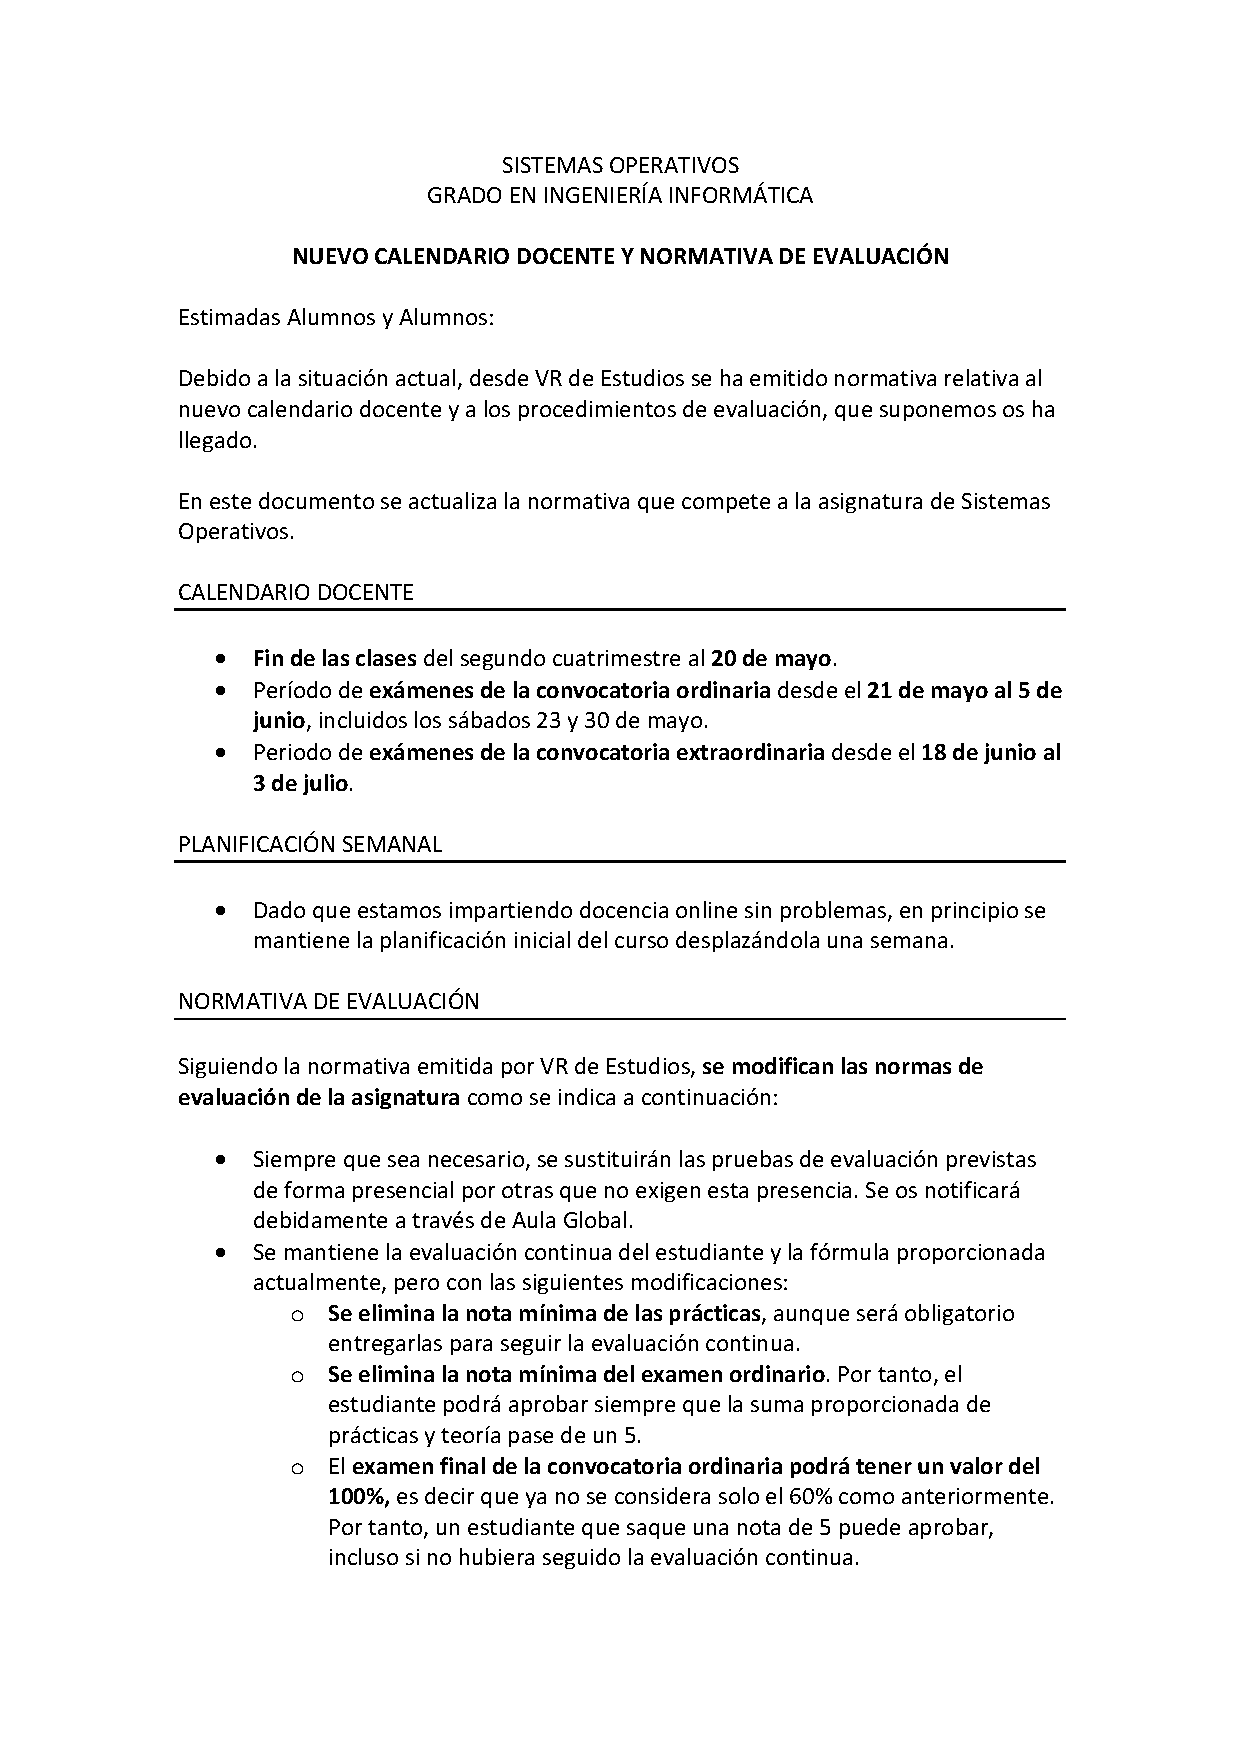
\includepdf[pages=-]{docs/Normativa-nueva.pdf}
\includepdf[pages=-]{docs/Sistemas_Operativos-2019-cronogramas.pdf}

\includepdf[pages=-]{docs/presentacion-ssoo.pdf}

\part{Resúmenes}
\chapter{Tema 1}
\section{Tema 1.1: Introducción a los Sistemas Operativos.}


  
  La función del sistema operativo es facilitar al usuario el uso del
  computador, antes solo se utilizaba para controlar y comunicarse con
  el hardware. Todas las funcionalidades y aplicaciones están sobre el
  sistema operativo.
  
  
  \textbf{Porque saber sobre SS. OO}:
  

  \begin{itemize}
  \item Influye en el funcionamiento, seguridad y rendimiento del
    computador. Por ello es importante conocer cómo funciona.
    
  \item Elegir el que mejor se adapte a nuestras necesidades o de la empresa
    es fundamental.
    

    \begin{itemize}
    \item Lo más importante, que sea rentable. Hay que proteger la
      inversión.
      
    \item Encontrar administradores que sepan sobre el sistema.
      
    \item Que ofrezca soporte y se actualice.
      
    \end{itemize}
  \item Al desarrollar aplicaciones saber como se comportará y comprender
    los problemas.
    

    \begin{itemize}
    \item Conocer los servicios que ofrece y como invocarlos. Y el
      desarrollo multi-hilo.
      
    \end{itemize}
  \end{itemize}
  
  No tener ideas preconcebidas de los SS. OO, ``ser agnóstico'',
  utilizar el que mejor se adapte a lo que necesito, hacer una checklist
  y ver cuál cumple más.
  
  
  LECTURA CAPÍTULO 1, libro CARRETERO 2007. Conceptos arquitectónicos
  del computador.
  
  
  \textbf{Sistema Operativo:} Programa intermediario entre el usuario y
  el hardware. Oculta el hardware, pero lo controla para ofrecer
  servicios al usuario, el usuario y hardware son muy distintos.
  

  \begin{itemize}
  \item Ejecuta programas.
    
  \item Hace uso eficiente de recursos.
    
  \item Proporciona una visión de máquina virtual.
    
  \end{itemize}
\pagebreak
  \begin{itemize}
  \item \textbf{Funciones del Sistema Operativo:}
    

    \begin{itemize}
    \item \textbf{Gestor de recursos}:
      

      \begin{itemize}
      \item Asigna y recupera recursos, como es la memoria.
        
      \item Protege al usuario, controla el acceso y los permisos de los
        usuarios.
        
      \item Contabiliza y monitoriza los recursos del sistema para ver como
        esta y que le pasa.
        
      \end{itemize}
    \item \textbf{Máquina extendida (servicios):}
      

      \begin{itemize}
      \item Ejecución de programas.
        
      \item Órdenes de E/S, leer/escribir, abrir/cerrar.
        
      \item Operación sobre archivos.
        
      \item Detección y tratamiento de errores, para que se reconozca y
        resuelvan.
        
      \end{itemize}
    \item \textbf{Interfaz de usuario:}
      

      \begin{itemize}
      \item Shell, es una interfaz gráfica externa al sistema operativo.
        
      \end{itemize}
    \end{itemize}
  \item \textbf{Niveles del Sistema Operativo}, los 3 principales:
    

    \begin{itemize}
    \item Usuario.
      
    \item Shell.
      
    \item Llamadas al sistema o Servicios.
      
    \item Núcleo/Kernel. Se ha ido reduciendo el Kernel y ampliando los
      Servicios
      
    \item Firmware/HardwareAbstractLogic, entre Kernel y Hardware.
      
    \item Hardware.
      
    \end{itemize}
  \item \textbf{Modos de ejecución}:
    

    \begin{itemize}
    \item Modo \textbf{usuario}: Está restringido, no puede acceder a
      ciertas aplicaciones, E/S, etc. Para proporcionar más seguridad.
      
    \item Modo \textbf{núcleo}: Puede ejecutar cualquier aplicación, sin
      restricciones. Más ``peligro''.
      
    \end{itemize}
  \item Los procesos y el sistema operativo, tienen espacios memoria
    reservada separados, y el del sistema operativo no es accesible para
    el usuario.
    
  \item Cuando un proceso necesita un servicio, se hace con una llamada al
    sistema, y el sistema lleva a cabo la función de la llamada.
    
  \item \textbf{Modificar el sistema operativo:} Principalmente para añadir
    funcionalidades o nuevo \textbf{hardware}. Pero se deben seguir unos
    estándares para asegurar que las aplicaciones funcionen en sistemas
    que sigan el mismo estándar.
    
  \end{itemize}
  
  \textbf{Sistemas operativos monolíticos}: No hay estructura clara y
  bien definida, pero es más eficiente, aunque su mantenimiento es más
  difícil. Todos los módulos se pueden llamar entre ellos. Siempre modo
  núcleo y todo enlazado en un ejecutable.
  
  
  \textbf{Sistemas operativos estructurados por capas:} Organizado por
  capas superpuestas, con una interfaz clara y bien definida. Una capa
  se apoya en la inferior, resulta menos eficiente, pero todo está más
  restringido y es más fácil el desarrollo y depuración.
  
  
  \textbf{Sistemas operativos estructurados cliente/servidor:} Consiste
  en implementar la mayor parte del sistema operativo como procesos de
  usuario, y una pequeña parte corre en modo núcleo llamado microkernel.
  Muy flexible, ya que funciona como pequeños programas.
  
  
  \textbf{Clasificación de Sistemas Operativos:}
  \vspace{-0.5cm}

  \begin{itemize}
  \item Número de procesos simultáneos:
    

    \begin{itemize}
    \item Monotarea: Un solo proceso a la vez.
      
    \item Multitarea: Varios procesos a la vez, necesita planificación.
      
    \end{itemize}
  \item Modo de interacción:
    

    \begin{itemize}
    \item Interactivo: Permite ejecutar procesos y obtenemos la solución en
      el momento.
      
    \item Por lotes: Tú pides al sistema y no sabes cuando se hará.
      
    \end{itemize}
  \item Número de usuarios simultáneos:
    

    \begin{itemize}
    \item Monousuario.
      
    \item Multiusuario.
      
    \end{itemize}
  \item Numero de procesadores:
    

    \begin{itemize}
    \item Monoprocesador.
      
    \item Multiprocesador: Son actualmente casi todos. Multicore.
      
    \end{itemize}
  \item Número de hilos:
    

    \begin{itemize}
    \item Monothread.
      
    \item Multithread.
      
    \end{itemize}
  \item Tipo de uso:
    

    \begin{itemize}
    \item Cliente: Pedir procesos.
      
    \item Servidor: Encargarse de los procesos.
      
    \item Empotrados: Dentro de un sistema cerrado, con unas funciones
      determinadas.
      
    \item Tiempo real: Se usan otros sistemas operativos para gestionarlos,
      otra planificación.
      
    \end{itemize}
  \end{itemize}
  
  \textbf{Arranque del sistema operativo}:
  

  \begin{itemize}
  \item Comienza con el envío de la interrupción de RESET (la 0), que carga
    el cargador (booter) y este carga la BIOS (Basic Input Output
    System) en memoria, la BIOS hace una comprobación del hardware (los
    periféricos, los discos, la memoria...) y cuando termina comienza a
    cargar en memoria el sistema operativo del disco que sabe que lo
    almacenaba. Una vez cargado el sistema operativo, se empieza a
    ejecutar, lo instala todo, y cuando ha terminado el sistema ya está
    ejecutado y se puede liberar la memoria que ocupaba para el usuario.
    

    \begin{itemize}
    \item Reset, pone los valores predefinidos a los registros y carga el
      cargador/booter.
      
    \item Se carga la BIOS, hace comprobaciones y cargar el sistema
      operativo en memoria.
      
    \item Se ejecuta el cargador del sistema operativo, que empieza a
      instalar el sistema y cuando termina el sistema ya está ejecutado,
      y se libera la memoria del cargador.
      
    \end{itemize}
  \end{itemize}
  
  \textbf{Parada del computador (Shutdown):} Procesos inversos al
  arranque.
  

  \begin{itemize}
  \item Al apagar, se vuelca la información a disco y se terminan todos los
    procesos.
    
  \item Si hay apagado brusco, se pierde información y se puede dañar, para
    evitarlo hay una pequeña batería que permite que se apague
    correctamente. Para sistemas grandes SAI.
    
  \item Otras alternativas son: Hibernación y Apagado en espera(Standby).
    
  \end{itemize}

\section{Tema 1.2: Servicios del SO.}

\begin{itemize}
\item \textbf{Ejecución del sistema operativo:} Una vez finalizado el
  arranque del sistema, el sistema solo se ejecuta como respuesta a
  interrupciones. Como son:
  

  \begin{itemize}
  \item Petición de servicio, están sobre el sistema operativo y no afectan
    a la máquina. lp\underline{d} d=daemon=demonio
    
  \item Interrupción de periféricos o reloj.
    
  \item Excepción de hardware.
    
  \end{itemize}
\item \textbf{Fases en la activación del Sistema Operativo:} Lo primero que
  se ejecuta es el proceso \underline{init} y a raíz de este van
  apareciendo más procesos que cuelgan de el, como si fuera un árbol del
  que van saliendo ramas. Al cambiar de proceso debe encontrarse tal y
  como estaba antes del cambio, eso se llama \underline{contexto}. Antes
  de cambiar se almacena todo del proceso actual e inmediatamente
  después se cargan los datos del otro. Todo proceso tiene su contexto.
  Se aprovechan los tiempos de espera(de cualquier proceso) para cambiar
  de proceso y ejecutar mientras tanto otras cosas, estos cambios los
  controla el \underline{planificador} y es \underline{concurrencia}.
  
\item \textbf{Activación de servicios:} Lo primero es pasar de modo usuario
  a modo núcleo, en la llamada el sistema tiene control total de la
  máquina. Ese cambio de privilegios es gracias a las bibliotecas que
  tienen acceso a superusuario. Y esos privilegios pueden ocasionar
  problemas de seguridad. Con la interrupción software trap se activa el
  modo seguro del sistema operativo.
  

  \begin{itemize}
  \item La rutina de bibliotecas es: Preparar la llamada al SO, instrucción
    trap y procesar los datos recibidos de la llamada.
    
  \end{itemize}
\item \textbf{Llamadas al sistema}:
  

  \begin{itemize}
  \item Interfaz entre aplicaciones y SO.
    
  \item Servicios típicos
    

    \begin{itemize}
    \item Gestión de procesos.
      
    \item Gestión de procesos ligeros: Si se crea, que se pueda controlar y
      matar.
      
    \item Gestión de señales y temporizador: Avisos y automatizaciones.
      
    \item Gestión de memoria.
      
    \item Gestión de ficheros y directorios.
      
    \end{itemize}
  \end{itemize}
\item \textbf{Bibliotecas}: Agrupación de funciones completas
  
\item \textbf{Invocación de la llamada:} Cada función de la interfaz de
  programación(API) se corresponde con algún servicio del sistema
  operativo. Incluye la ejecución de trap que transfiere el control al
  sistema operativo con una interrupción, el sistema operativo trata la
  interrupción y devuelve el control al programa de usuario.
  

  \begin{itemize}
  \item Salta a la librería, comprueba y almacena los parámetros necesarios
    para la operación, se pueden pasar en registros, tabla de memoria o
    en pila. Pone el número de operación, el identificador numérico
    correspondiente y hace syscall (trap), para llamar al sistema a
    ejecutar esa operación.
    
  \item El SO ejecuta internamente la operación, recibe el identificador que
    le indica la dirección de la rutina de tratamiento y la ejecuta, y
    devuelve 0 si ha funcionado o -1 si ha fallado.
    
  \item Resuelta la operación, vuelve al código del usuario con el valor
    esperado.
    
  \end{itemize}
\item \textbf{Interfaz del programador:} Ofrece una visión que como máquina
  extendida tiene el usuario del sistema, cada sistema operativo puede
  ofrecer uno o varias.
  
\item \textbf{Estándar POSIX (Portable Operative System Interface for X)}:
  Interfaz estándar de sistema operativo de IEEE. El objetivo es que
  todas la maquinas que compartan este estándar puedan ejecutar los
  mismos programas, portabilidad.
  

  \begin{itemize}
  \item Nombres de funciones cortos y en letras minúsculas, representativos
    y en ingles.
    
  \item Normalmente el éxito devuelve 0 y en caso de error -1. errno=error
    number y perror(errno) nos dice que error es y nos proporciona algo
    de información.
    
  \end{itemize}
\item \textbf{Ejecución de un mandato en Shell}: Lo que hace cada vez, hay
  una relación jerárquica de procesos shell, que permite que en caso de
  error el proceso shell padre no muera.
  

  \begin{itemize}
  \item Lo primero el padre ejecuta fork(), que crea un duplicado del padre
    que funcionará a la vez que el padre y ese hijo se identifica por un
    pid(process id) de 0 y el padre tendrá otro cualquiera. Cuando se
    ejecuta fork el hijo siempre es pid=0.
    
  \item Para que sea el hijo el que ejecute el mandato y corra el peligro de
    error, y no el padre. Lo que se hace es que el proceso con ID 0, el
    hijo, ejecute el mandato con execvp(,) y si da error ese proceso
    hijo muere y queda vivo el padre, pero si no falla ambos seguirán
    vivos hasta el final del programa. Se hace un switch, si pid del
    hijo es -1 ha habido un problema al crearlo y termina, si es 0
    ejecuta el mandato y break y si no es ninguno de los anteriores es
    el padre.
    
  \end{itemize}
\item \textbf{Servicio fork()}: Devuelve un pid\_t que es el ID del proceso,
  en el padre el valor es el identificador del hijo y en el hijo el
  valor es 0, y -1 en caso de fallo. Su función es duplicar el proceso
  que invoca la llamada, tanto el proceso hijo como el padre siguen
  ejecutando el mismo programa. El proceso hijo conservará una
  \underline{copia} exactamente igual de todo lo que tenía el padre.
  
\item \textbf{Servicio wait(\&status):} Bloquea la ejecución del padre hasta
  que el proceso hijo muere, devuelve el identificador del proceso que
  ha finalizado, y status es el valor que devuelve el hijo cuando llama
  al exit().
  
\item \textbf{Servicio exec:} Ejecuta un programa en ese proceso, el proceso
  recibe toda la información y cambia su imagen, desaparece el código
  que tiene y se sustituye por el del programa si ha ido bien, si no
  retorna -1. Cuando se hace exec la tabla de ficheros abiertos no se
  borra. Servicio único para múltiples funciones de biblioteca. Recibe
  como primer argumento el nombre de la función a ejecutar y el resto
  son los parámetros del main. execlp(`ls','ls','-l')
  \pagebreak
\item \textbf{Servicio exit (void exit(status)):} Finaliza la ejecución del
  proceso, se escribe al final de un programa o al detectar un error. Se
  cierran todos los descriptores de ficheros abiertos y se liberan todos
  lo recursos del proceso. Devolver negativo es indicativo de error y 0
  de que la ejecución ha ido correctamente, pero también puede tomar
  otros valores. Todos lo valores que toma status sirven para dar
  información adicional de como ha ido la ejecución. return 0=exit(0)
  
\item \textbf{Fichero}, es una manera de almacenar información de una manera
  más persistente, para reutilizarlos o simplemente para tenerlos.
  
\item \textbf{Operaciones genéricas sobre ficheros}: AMPLIAR
  

  \begin{itemize}
  \item Crear: creat(nombre, O\_WRONLY\textbar O\_CREAT\textbar O\_TRUNC,
    mode);
    
  \item Borrar: unlink(nombre);
    
  \item Abrir: open(descriptor, permisos); O\_RDWR/WRONLY/RDONLY/APPEND
    sigue al final del fichero.
    
  \item Cerrar: close(descriptor);
    
  \item Leer: read(descriptorLectura, buffer, tamañoALeer);
    
  \item Escribir: write(descriptorEscritura, buffer, longitudAEscribir);
    
  \item Posicionar: lseek(descriptor, desplazamiento, dondeComenzar);
    SEEK\_SET/END/CUR
    
  \item Control: fnctl para modificación de atributos, dup para duplicar
    descriptores de fichero, ftruncade asignación de espacio a un
    fichero, stat información sobre un fichero, utime para alterar los
    atributos de fecha.
    
  \end{itemize}
\end{itemize}

\chapter{Tema 2}
\section{Tema 2.1: Introducción a la gestión de Procesos.}

\textbf{Proceso:} Programa en ejecución, cada ejecución da lugar un
  proceso nuevo. Cada proceso tiene un identificador único llamado
  pid(process id), que nos permite obtener más información sobre el
  proceso, como el contexto, directorio, padre, etc.
  

  \begin{itemize}
  \item Está formado por: Código del programa(instrucciones) y los datos
    asociados a la propia ejecución del programa.
    
  \item \textbf{Partes}: Pila(se va ampliando hacia abajo), memoria
    dinámica, datos(se amplía hacia arriba) y texto(el código). Cada
    proceso tiene esta estructura y son independientes entre ellos.
    
  \end{itemize}
\textbf{Ciclo de vida de un proceso:}
  

  \begin{itemize}
  \item \textbf{Listo}: Cuando se ejecuta un programa se hace el exec, lo
    primero que hace es comprobar sus propiedades y si se tiene recursos
    para ejecutar ese proceso nuevo. Si se tienen recursos se creará ese
    proceso nuevo y se le da un pid propio, el pid debe estar por debajo
    del límite máximo de procesos o no se podrá crear. No se reutilizan
    pid's, habría que reiniciar.
    
  \item \textbf{En ejecución:} Cuando está listo, se pasa a memoria y se
    ejecuta, si es para algo lento lo pasaremos ha bloqueado, para que
    espere a recibir los datos que necesite, y pasara a listo, si el
    proceso ha superado su tiempo asignado o si cede su CPU. Este último
    lo controla el planificador. El proceso puede terminar con exit, que
    liberará los recursos o si no, esperará un tiempo antes de
    liberarlo.
    
  \item \textbf{Bloqueado}: Cuando el proceso está esperando a recibir
    datos, si lo recibe pasa a listo, pero si no recibe los datos en
    ningún momento se quedará en bloqueado.
    
  \end{itemize}
\textbf{Modelo de colas simplificado: Un procesador}.
  

  \begin{itemize}
  \item Los procesos están en una cola, y según las unidades de procesado
    que necesita va a una parte u otra, hay una para procesos rápidos y
    otras para procesos más pesados. Si un proceso en su franja de
    tiempo no ha terminado, se vuelve a poner en la cola. El que elige
    donde va cada proceso es el dispatcher. (Función como la cola de un
    supermercado)
    
  \end{itemize}
  \pagebreak
\textbf{Información de un proceso}: Toda la información que permite la
  correcta ejecución del proceso.
  

  \begin{itemize}
  \item \textbf{Tres categorías}:
    

    \begin{itemize}
    \item Información almacenada en el procesador.
      
    \item Información almacenada en memoria.
      
    \item Información adicional gestionada por el sistema operativo.
      
    \end{itemize}
  \item El pid se almacena en la tabla de procesos (TP). Cada proceso tiene
    su BCP, donde se almacena su entorno(no cambia), mapa de
    memoria(texto y datos) y el contexto/estado(puede cambiar).
    
  \item En el estado/contexto se incluye los valores de los registros
    accesibles y no accesibles para el usuario del procesador. Cuando se
    cambia de contexto, se salvaguarda el estado del procesador del
    saliente y se restaura el estado del proceso del entrante.
    
  \item \textbf{Memoria virtual}: Se engaña al sistema, ya que se necesitan
    recursos que no tiene la máquina y puede que tenga que matar a otro
    proceso para ir haciendo hueco. Mem. dinam.
    
  \item \textbf{Modelo de imagen de memoria con Regiones múltiples:}
    

    \begin{itemize}
    \item El número de regiones es fijo, y cada región es de tamaño
      variable.
      
    \item Las regiones son: \underline{Pila, Datos y Texto.}
      
    \item Con memoria virtual el hueco entre pila y datos no consume
      recursos físicos.
      
    \end{itemize}
  \item Pero hay modelos de imagen de memoria con una sola región y también
    con regiones no fijas, que son opciones más avanzadas como Windows.
    
  \item \textbf{El sistema operativo} mantiene información adicional sobre
    los procesos, en la Tabla de Procesos. \underline{Cada una de las
    entradas de la TP es un BCP} (Bloque de Control de Procesos), que
    mantiene casi toda la información sobre el proceso.
    

    \begin{itemize}
    \item \textbf{Contenido del BCP:}
      

      \begin{itemize}
      \item Información de identificación:
        

        \begin{itemize}
        \item Estado del proceso.
          
        \item Evento por el que espera, si es que está bloqueado.
          
        \item Prioridad del proceso.
          
        \item Información de planificación.
          
        \end{itemize}
		\pagebreak
      \item Estado del procesador:
        

        \begin{itemize}
        \item Archivos abiertos.
          
        \item Puertos de comunicación usado
          
        \item Temporizadores
          
        \end{itemize}
      \item Información de control del proceso:
        

        \begin{itemize}
        \item Punteros para estructurar los procesos en cola.
          
        \end{itemize}
      \end{itemize}
    \item \textbf{Contenido fuera del BCP}:
      

      \begin{itemize}
      \item El BCP no almacena toda la información del un proceso, se decide
        que no almacenar según la eficiencia, si se puede almacenar bien
        o no en la tabla, y si hay que compartir información, si se
        comparte algún dato no estará en el BCP.
        
      \item Se usan punteros, que se almacenan en tablas de páginas, y desde
        el BCP se puede acceder a esa tabla. Se usa este método porque
        tienen tamaños variables y el compartir datos debe ser externo.
        
      \end{itemize}
    \item La tabla de punteros de posición de los ficheros, que almacena los
      ficheros abiertos por un proceso, se almacena fuera del BCP y si se
      almacena dentro no podrán ser compartidos.
      
    \end{itemize}
  \item \textbf{El servicio fork,} hace que el proceso padre e hijo
    compartan el contexto, y solo se hará una copia cuando el hijo haga
    una modificación, mientras comparte el espacio con el padre.
    
  \item \textbf{El servicio exec,} lee un ejecutable, y cambia el mapa de
    memoria y el contexto, al proceso que lo está ejecutando.
    
  \item \textbf{El servicio exit,} finaliza la ejecución del proceso, cierra
    los descriptores, liberan todos los recursos y libera el BCP. Los 3
    están explicados en el Tema 1.
    
  \end{itemize}
\textbf{Tipos de sistemas operativos:}
  

  \begin{itemize}
  \item \textbf{Multiproceso}: Utiliza el paralelismo, varios procesos
    funcionan a la vez.
    

    \begin{itemize}
    \item Multiusuario y Monousuario.
      
    \end{itemize}
  \item \textbf{Monoproceso}: Concurrencia, funciona un proceso a la vez,
    pero se van compaginando y da la sensación de paralelismo
    

    \begin{itemize}
    \item Monousuario.
      
    \end{itemize}
  \end{itemize}
  \pagebreak
\textbf{Multitarea}: Alternancia en los procesos de fases de E/S y de
  procesamiento, la memoria almacena varios procesos.
  

  \begin{itemize}
  \item \textbf{Ventajas}:
    

    \begin{itemize}
    \item Facilita la programación, se divide un programa en procesos.
      Modularidad.
      
    \item Permite el servicio interactivo simultáneo de varios usuarios.
      
    \item Aprovecha los tiempos de espera de E/S de los procesos.
      
    \item Aumenta el uso de CPU.
      
    \end{itemize}
  \item \textbf{Grado de multiprogramación:} Numero de procesos activos,
    cuantos más procesos el rendimiento de la máquina disminuye. Los
    sistemas con memoria virtual dividen el espacio direccionable de los
    procesos en páginas y el de memoria física en marcos de página. El
    numero de páginas en memoria principal es el \underline{Conjunto
    Residente.}
    

    \begin{itemize}
    \item Cuando aumenta el grado de multiprogramación, disminuye el tamaño
      del conjunto residente de cada proceso, para que quepan todos.
      

      \begin{itemize}
      \item \textbf{Con poca memoria física:} Se produce hiperpaginación
        cuando alcanzo alto porcentaje de uso, para solucionarlo hay que
        ampliar la memoria principal.
        
      \item \textbf{Con mucha memoria física}: Se alcanza alto porcentaje de
        utilización de CPU con menos procesos de los que caben en
        memoria, para solucionarlo se puede mejorar el procesador o
        añadir más procesadores.
        
      \end{itemize}
    \end{itemize}
  \end{itemize}
\textbf{Cambio de contexto}: Cuando se pasa de ejecutar un proceso a
  otro. Se produce cuando el sistema operativo asigna el procesador a un
  nuevo proceso.
  

  \begin{itemize}
  \item \textbf{Tipos de cambios de contexto:}
    

    \begin{itemize}
    \item \textbf{Cambio de contexto voluntario(CCV):} El proceso realiza
      una llamada al sistema o produce una excepción que implica esperar
      por un evento, así deja funcionar a otro.
      
    \item \textbf{Cambio de contexto involuntario(CCI)}: El SO quita de la
      CPU al proceso, puede darse porque el proceso haya agotado su
      rodaja de ejecución.
      
    \end{itemize}
  \item \textbf{Acciones}:
    

    \begin{itemize}
    \item Guarda el estado del procesador en el BCP del proceso en
      ejecución.
      
    \item Restaurar el estado del nuevo proceso en el procesador.
      
    \end{itemize}
  \end{itemize}
Generación de ejecutables: MIRAR LIBRO Y DIAPOSITIVA.

\section{Tema 2.2: Planificación de procesos.}

\textbf{Creación de procesos en UNIX:} Se distingue entre crear
  procesos y ejecutar nuevos programas.
  

  \begin{itemize}
  \item Para crear un proceso se hace mediante fork(), que no cambia la
    imagen de memoria y mantiene los valores del padre, crea una copia,
    y los cambios en el hijo no le afectan. Copia el BCP del padre y su
    Mapa de memoria (incluyendo pilas).
    

    \begin{itemize}
    \item Un inconveniente es que muchos datos podrían compartirse.
      
    \end{itemize}
  \item Para ejecutar un programa se hace mediante exec(), se hace sobre
    procesos hijo, sustituye su imagen en memoria por la del programa.
    Mientras el padre puede esperar al hijo con wait o seguir creando
    hijos.
    

    \begin{itemize}
    \item Un inconveniente es que fork ha copiado todo lo del padre, para
      que luego lo deshecha el exec.
      
    \end{itemize}
  \item Para solucionar ambos inconvenientes se usa COW(Copy-on-Write), los
    datos se marcan de manera que si se intentan modificar se realiza
    una copia para cada proceso.
    
  \end{itemize}
\textbf{Terminación de procesos:} Todos los recursos asignados son
  liberados, excepto el valor del exit que se mantiene en el BCP
  esperando el wait del padre y si el padre ha muerto (el hijo se queda
  zombi) lo hereda el init y este hace el wait. Entonces se elimina el
  BCP, tras el wait. Puede terminar de 2 maneras:
  

  \begin{itemize}
  \item \textbf{Voluntariamente}: Llamada al sistema exit().
    
  \item \textbf{Involuntariamente}: Excepciones, abortado por el
    usuario(ctrl+c) u otro proceso(kill).
    
  \end{itemize}
\textbf{Expulsión a disco(swap):} Cuando hay demasiados procesos y
  baja el rendimiento, se pasan algunos procesos a disco con swap que
  libera memoria, y cuando se quieran seguir ejecutando se pasa de nuevo
  a memoria. Los nuevos estados son: Bloqueado y suspendido, y Listo y
  suspendido.
  
\textbf{Niveles de planificación:}
  

  \begin{itemize}
  \item Planificación a corto plazo: Selecciona el siguiente proceso a
    ejecutar.
    
  \item Planificación a medio plazo: Elegir que proceso se retira o añade a
    memoria principal.
    
  \item Planificación a largo plazo: Realiza el control de admisión de
    procesos a ejecutar.
    
  \end{itemize}
\textbf{Tipos de planificación:}
  

  \begin{itemize}
  \item \textbf{No apropiativo:} El proceso conserva el uso de CPU, no se
    puede expulsar hasta que termine.
    
  \item \textbf{Apropiativo:} El sistema puede expulsar a un proceso de CPU,
    se puede expulsar, aunque no haya terminado para ejecutar otro
    proceso.
    
  \end{itemize}
\textbf{Momentos de decidir la planificación:}
  

  \begin{itemize}
  \item Cuando un proceso se bloquea, mientras espera el evento se pasa a
    ejecutar otro proceso.
    
  \item Cuando se produce una interrupción, como la del reloj o de E/S.
    
  \item Cuando termina un proceso.
    
  \end{itemize}
\textbf{Cola de procesos:} Los procesos listos para ejecutar se
  mantiene en una cola, que puede ser única, por tipo de proceso o por
  prioridad. Cuando se saca un proceso que no ha terminado se pone al
  final de la cola. Si entra a ejecutar uno nuevo se pone antes que el
  que está terminando.
  
\textbf{Algoritmos de planificación:}
  

  \begin{itemize}
  \item Se pueden orientar a:
    

    \begin{itemize}
    \item \textbf{Utilización de CPU:} maximizar el tiempo de uso.
      
    \item \textbf{Productividad:} maximizar el número de procesos que
      terminan por unidad de tiempo.
      
    \item \textbf{Tiempo de retorno(Tq=Tf-Ti):} Minimizar el tiempo que un
      proceso pasa desde que entra hasta que termina.
      
    \item \textbf{Tiempo de servicio(Ts):} Tiempo que se ha dedicado a
      tareas productivas.
      
    \item \textbf{Tiempo de espera(Te):} Tiempo que un proceso ha estado en
      la cola de espera.
      
    \item \textbf{Tiempo de retorno normalizado(Tn=Tq/Ts):} Tanto por uno
      que un proceso ha estado en espera.
      
    \end{itemize}
  \item \textbf{Asignación First to Come First to Serve (FCFS):} Es FIFO,
    primero en llegar primero en salir. Es no apropiativo, no se puede
    expulsar un proceso. Penaliza a los cortos, que tienen que esperar a
    que terminen todos los previos.
    
  \item \textbf{Asignación Shortest Job First:} Primero los procesos más
    cortos, menor tiempo de servicio. Es no apropiativo, no se puede
    expulsar un proceso. Se debe conocer la duración de antemano. El
    problema es que si solo llegan procesos cortos los largos no se
    ejecutan.
    
  \item \textbf{Cíclico o Round-Robin:} Mantiene una cola FIFO con los
    procesos listos para ejecutar. A cada proceso se le asigna una
    rodaja de tiempo de procesador, cuando la agota pasa a la cola y se
    ejecuta el siguiente en la cola. Se ejecutan un poco todos, hasta
    que terminan. Un proceso puede volver a lista porque acabe su
    tiempo o pase ha bloqueado, esperando un evento. Es apropiativo, por
    eso se puede expulsar un proceso para poner otro a ejecutar.
    

    \begin{itemize}
    \item Hay que intentar que tampoco haya demasiados cambios de contexto,
      ya que estos añaden tiempo.
      
    \end{itemize}
  \item \textbf{Asignación por prioridades:} Cada proceso tiene una
    prioridad asignada, y se seleccionan primero los procesos con mayor
    prioridad.
    
  \end{itemize}


\section{Tema 2.4: Hilos y Procesos.}

Hilos de ejecución de un proceso de forma concurrente. Los threads de
  un proceso se guardan en su BCP en la tabla de threads, Threads Table,
  donde se almacena su información y contenido. Se considera la unidad
  básica de utilización de la CPU.
  
\textbf{Crear hilos permite que:}
  

  \begin{itemize}
  \item Compartan memoria entre ellos, pero cada uno necesita una pila para
    almacenar sus datos y un minicontexto propio.
    
  \item Aprovechen mejor la rodaja de tiempo que tienen asignada, al hacer
    menos cambios de contexto, que los que implica crear y terminar un
    proceso hijo.
    
  \item Un thread está ligado a un proceso, no es independiente por lo que
    si muere el proceso mueren los hilos, no como pasa con los procesos
    hijos.
    
  \end{itemize}
\textbf{Contenido de un hilo:}
  
\vspace{-0.5cm}

  \begin{itemize}
  \item Identificador del thread.
    
  \item Contador de programa.
    
  \item Conjunto de registros.
    
  \item Pila.
    
  \end{itemize}
\textbf{Comparten entre hilos:}
\vspace{-0.5cm}


  \begin{itemize}
  \item Mapa de memoria.
    
  \item Ficheros abiertos.
    
  \item Señales, semáforos y temporizadores.
    
  \end{itemize}
\textbf{Beneficios:}
  

  \begin{itemize}
  \item Mayor interactividad al separar las tareas en hilos.
    
  \item Comparten la mayor parte de los recursos.
    
  \item Cuesta menos tiempo crear un hilo que un proceso.
    
  \item En arquitecturas multiproceso permite hacer ejecución en paralelo
    asignando hilos distintos a distintos procesadores.
    
  \end{itemize}
\textbf{Soporte de hilos:}
  

  \begin{itemize}
  \item \textbf{Espacio de usuario, ULT}, User Level Threads.
    

    \begin{itemize}
    \item Están implementados en forma de biblioteca de funciones.
      
    \item El kernel no tiene conocimiento sobre los threads, solo sobre el
      proceso creador.
      
    \item Es más rápido, pero un bloqueo bloquea todo el proceso.
      
    \item Un hilo de usuario se puede pasar al kernel para que esté lo
      gestione, y deja de depender del proceso y aunque muera el proceso
      no muere el hilo. Cambia su id.
      
    \end{itemize}
  \item \textbf{Espacio de núcleo, KLT}, Kernel Level Threads.
    

    \begin{itemize}
    \item Son de los que se ocupa el kernel, de crearlos, planificarlo y
      destruirlos.
      
    \item Un poco más lentos al hacerlo por medio del kernel y no
      directamente.
      
    \item Los bloqueos solo bloquean el thread implicado, no a todo.
      
    \item Se pueden ejecutar varios procesos a la vez, pero hay un límite de
      threads.
      
    \end{itemize}
  \end{itemize}
\textbf{Modelos de múltiples hilos:}
  

  \begin{itemize}
  \item \textbf{Muchos a uno:} Corresponden muchos hilos de usuario con un
    único hilo del núcleo. Una llamada bloqueante bloquea todos los
    hilos.
    
  \item \textbf{Uno a uno:} Hace corresponder un hilo del kernel a cada hilo
    de usuario. La mayoría de las implementaciones restringen al numero
    de hilos que se pueden crear.
    
  \item \textbf{Muchos a muchos:} Multiplexa los threads de usuario en un
    numero determinado de threads en el kernel. El núcleo se complica
    mucho.
    
  \end{itemize}
  \pagebreak
\textbf{Aspectos de diseño:}
  

  \begin{itemize}
  \item Cuando se hace fork de un proceso con hilos, duplica el proceso con
    todos sus hilos.
    
  \item exec no es adecuado, sustituirá la imagen del proceso, que quitará
    todo incluido los hilos.
    
  \item \textbf{Otra versión:} Cuando hace fork, duplica el proceso solo con
    el hilo que hace fork.
    
  \item Esta versión es más eficiente si va a hacer un exec.
    
  \end{itemize}

  \begin{itemize}
  \item \textbf{Cancelación de hilos:} Un hilo notifica a otro de que deben
    terminar.
    

    \begin{itemize}
    \item \textbf{Cancelación asíncrona:} Se fuerza la terminación
      instantánea del hilo.
      

      \begin{itemize}
      \item Puede ocasionar problemas con los recursos asignados.
        
      \end{itemize}
    \item \textbf{Cancelación diferida:} El hilo comprueba periódicamente si
      debe terminar. Es preferible.
      
    \end{itemize}
  \item Para aplicaciones que reciben peticiones y las procesan se pueden
    usar hilos.
    

    \begin{itemize}
    \item Se hace \textbf{Thread Pool (Conjunto de Hilos)} que consiste en
      crear con anterioridad los hilos para evitar el tiempo de creación
      (retardos) y se dejan en espera, y se establece un límite, para
      intentar evitar que una avalancha de peticiones agote los recursos
      del sistema. Cuando se reciben más peticiones de las que se pueden
      tratar se ponen en cola y cuando la cola se ha llegado se hace
      denegación de servicios, que no la deja entrar mientras no vayan
      acabando las peticiones.
      
    \end{itemize}
  \end{itemize}
\textbf{Hilos en pthreads:}
  

  \begin{itemize}
  \item \textbf{Creación de hilos:}
    

    \begin{itemize}
    \item int pthread\_create(pthread\_t *thread, const pthread\_attr\_t
      *attr, void *(*func)(void *), void *arg)
      

      \begin{itemize}
      \item Devuelve un entero que indica como ha ido la ejecución.
        
      \item *thread es el puntero donde se almacenará el ThreadId, el
        manejador del hilo.
        
      \item *attr Estructura de atributos.
        
      \item *(*func)(void *) función con el código a ejecutar.
        
      \item *arg parámetro del hilo.
        
      \end{itemize}
	  \pagebreak
    \item Estructura pthead\_attr\_t: Son los atributos asociados a cada
      hilo.
      

      \begin{itemize}
      \item Controlan:
        

        \begin{itemize}
        \item Si el hilo es independiente o dependiente, de kernel o de
          biblioteca.
          
        \item Tamaño de la pila privada.
          
        \item Localización de la pila.
          
        \item Política de planificación, solo posible si es de kernel.
          
        \end{itemize}
      \item Inicializar: pthread\_attr\_init(pthread\_attr\_t *attr)
        
      \item Destruir: pthread\_attr\_destroy(pthread\_attr\_t *attr)
        
      \item Por defecto el atributo de independencia está en
        PTHREAD\_CREATE\_JOINABLE, lo que quiere decir que espera un
        join y no se liberan los recursos. La otra opción cuando acaba
        el sistema operativo libera los recursos. PT...\_DETACHED.
        
      \item El resto en diapositiva 28 de Tema 2.3.
        
      \end{itemize}
    \item pthread\_t pthread\_self(void) Devuelve el identificador del
      thread.
      
    \item int pthread\_join(pthread\_t thread, void **value) Es el wait de
      los hilos.
      

      \begin{itemize}
      \item thread manejador del hilo a esperar.
        
      \item **value Valor de terminación del hilo.
        
      \end{itemize}
    \item int pthread\_exit(void *value) Finaliza su ejecución y devuelve
      value que puede ser de cualquier tipo. Aunque no hagan join, no se
      quedan hilos zombis.
      
    \item \textbf{EVITAR usar variables globales, fork y exec.}
      
    \end{itemize}
  \end{itemize}
\textbf{Planificación de hilos:} Se basa en el modelo de prioridades y
  no utiliza el modelo de segmentación por segmentos de tiempo. Un
  thread continuará ejecutándose en la CPU hasta pasar a un estado que
  no le permita seguir en ejecución. Para alternar entre thread, se debe
  asegurar que el thread permita la ejecución de otros threads.
  

  \begin{itemize}
  \item PTHREAD\_SCOPE\_PROCESS Planificación PCS, del proceso del user, de
    biblioteca.
    
  \item PTHREAD\_SCOPE\_SYSTEM Planificación SCS, del kernel.
    
  \end{itemize}

\section{Tema 2.4 Señales}

\textbf{Señales}: Son un mecanismo para comunicar eventos a los
  procesos, para que estos puedan reaccionar. Son excepciones
  asíncronas, se procesan de inmediato. Posibles reacciones a una
  respuesta:
  

  \begin{itemize}
  \item Ignorar la señal, SIG\_IGN.
    
  \item Invocar la rutina de tratamiento por defecto, si el proceso no
    esperaba ninguna lo general es que sea muerte.
    
  \item Invocar a una rutina de tratamiento propia.
    

    \begin{itemize}
    \item Por ejemplo, un proceso padre recibe la señal SGCHLD cuando su
      proceso hijo termina, esa señal la envía el SO, no el hijo
      directamente.
      
    \end{itemize}
  \end{itemize}

  \begin{itemize}
  \item Son interrupciones al proceso, si está ejecutando normal la rutina
    se lleva a cabo en el siguiente ciclo de reloj y si se captura
    cuando termine continuara por donde estaba. Pero si está en un bucle
    se ejecuta en ese momento, ya que no se sabe cuando terminara el
    bucle.
    
  \item \textbf{Tratamiento}: El SO las transmite al proceso, pero el
    proceso debe estar preparado para recibirlo o en general muere. El
    proceso debe especificar con sigaction que señal espera y que rutina
    de tratamiento seguir.
    
  \item \textbf{Enviar señal a un proceso}: \textbf{int kill(pid\_t pid, int
    sig);} No es para matar el proceso, aunque si el proceso no la
    espera le matará.
    

    \begin{itemize}
    \item Para enviar una señal a sí mismo \textbf{int raise(int sig);}
      
    \item CTRL-C SIGINT
      
    \item CTRL-Z SIGSTOP
      
    \end{itemize}
  \item \textbf{Esperar a una señal:} Con el servicio \textbf{int
    pause(void)} el proceso espera hasta que le llegue una señal
    cualquiera que le reanuda, se utiliza para ejecutar en orden.
    

    \begin{itemize}
    \item No se puede especificar un plazo de desbloqueo.
      
    \item No se puede indicar el tipo de señal que se espera.
      
    \item No se desbloquea si recibe una señal ignorada.
      
    \end{itemize}
  \item \textbf{Sleep(unsigned int sec)} Suspende un proceso hasta que vence
    un plazo o se recibe una señal.
    
  \item \textbf{Especificar acción:} Se utiliza sigaction para especificar
    la acción a realizar como tratamiento de la señal sig. OJO, cuando
    se ha completado la rutina rearmar el sigaction.
    

    \begin{itemize}
    \item \textbf{int sigaction(int sig, struct sigaction *act, struct
      sigaction *oact);}
      

      \begin{itemize}
      \item Preferible ante signal(,)
        
      \item Sig es la señal para la que actúa.
        
      \item En la estructura de act, en sa\_handler se pone que rutina
        seguir.
        
      \item En oact está la configuración.
        
      \end{itemize}
	  \pagebreak
    \item \textbf{Estructura sigaction\{void (*sa\_handler)(); sigset\_t
      sa\_mask; int sa\_flags;\};}
      

      \begin{itemize}
      \item Sa\_handler Es el manejador, lo que hace, puede ser SIG\_DFL por
        defecto, SIG\_IGN ignora la señal o una dirección de una
        función.
        
      \item Sa\_mask Mascara de señales a ignorar durante el manejador.
        
      \item Sa\_flags Opciones.
        
      \end{itemize}
    \end{itemize}
  \item \textbf{Lista de señales importantes}: Están incluidas en signal.h,
    que son propias del sistema operativo.
    

    \begin{itemize}
    \item SIGILL Instrucción ilegal.
      
    \item SIGALRM Cuando termina un temporizador.
      
    \item SIGKILL Mata al proceso.
      
    \item SIGSGEV Violación de segmento de memoria.
      
    \item SIGUSR1 y SIGUSR2 Reservadas par el uso del programador.
      
    \end{itemize}
  \item \textbf{Conjunto de señales:}
    
  \end{itemize}
\textbf{Temporizadores:} El sistema operativo mantiene un temporizador
  por proceso, en su BCP.
  

  \begin{itemize}
  \item Es el sistema operativo quien actualiza todos los temporizadores.
    
  \item Cuando llega a cero el SO pasa al proceso la señal SIGALRM, para que
    se ejecute la rutina de tratamiento.
    
  \end{itemize}

  \begin{itemize}
  \item \textbf{Establecer un temporizador:} int alarm(unsigned int sec)
    puede cambiarse sec por otra unidad de tiempo. Si el parámetro es 0,
    desactiva el temporizador.
    
  \item \textbf{Diferencia de sleep y alarm:}
    

    \begin{itemize}
    \item \textbf{alarm}, es una llamada al sistema y del proceso se duerme
      exactamente el tiempo indicado, lo tiene medido.
      
    \item \textbf{sleep}, no es una llamada al sistema y como mínimo duerme
      el tiempo indicado.
      
    \end{itemize}
  \end{itemize}
\textbf{Excepciones}: Cuando el hardware detecta condiciones
  especiales; fallo de página, escritura a página de solo lectura,
  desbordamiento de pila, violación de segmento, syscall
  
  \vspace{-0.5cm}

  \begin{itemize}
  \item Transfiere control al SO para su tratamiento, que:
    

    \begin{itemize}
    \item Salva el contexto del proceso.
      
    \item Ejecuta la rutina si es necesario.
      
    \item Envía una señal al proceso indicando la excepción.
      
    \end{itemize}
  \item Sirven para optimizar el rendimiento, ya que ahorran código de
    comprobaciones.
    
  \item Muchos lenguajes usan mecanismos llamados Exceptions para controlar
    errores.
    
  \end{itemize}
\textbf{Entorno de un proceso}: Se hereda del padre y contiene los
  siguientes datos:
  

  \begin{itemize}
  \item Vector de argumentos del comando del programa
    
  \item Vector de entorno, una lista de variables que el padre pasa al hijo.
    \textless nombre, valor\textgreater{}
    

    \begin{itemize}
    \item Es una forma flexible de comunicar ambos procesos y determinar
      aspectos de la ejecución del hijo en modo usuario. Partícula a
      aspectos a nivel de cada proceso.
      
    \end{itemize}
  \end{itemize}

  \begin{itemize}
  \item \textbf{Variables de entorno:} Mecanismo de paso de información a un
    proceso.
    
  \item \textbf{Localización:} El entorno se coloca en la pila del proceso
    al iniciarlo. Y se recibe como tercer parámetro de main la dirección
    de la tabla de variables de entorno.
    
  \end{itemize}

\chapter{Tema 3}
\textbf{Tema 3.1: Procesos concurrentes y problema en la comunicación y
la sincronización.}

\textbf{Procesos concurrentes:} Dos procesos ejecutándose en el mismo
  momento, es decir, se ejecutan de manera que sus intervalos de
  ejecución se solapan. No que uno se pasó a otro.
  

  \begin{itemize}
  \item \textbf{Tipos de concurrencias:}
    

    \begin{itemize}
    \item \textbf{Concurrencia aparente:} Hay más procesos que procesadores,
      los procesadores se multiplexan en el tiempo. Pseudoparalelismo.
      
    \item \textbf{Concurrencia real:} Cada proceso se ejecuta en un
      procesador, se produce una ejecución en paralelo. Paralelismo
      real.
      
    \end{itemize}
  \item \textbf{Modelos de programación concurrente:}
    

    \begin{itemize}
    \item \textbf{Único procesador:} El sistema operativo se encarga de
      repartir el tiempo entre los procesos, incluso expulsándolos. Es
      inherente.
      
    \item \textbf{Multiprocesador}: Combinan paralelismo real con
      pseudoparalelismo. Ya que normalmente hay más procesos que
      procesadores.
      
    \item \textbf{Sistema distribuido:} Varios computadores conectados por
      red.
      
    \end{itemize}
  \item \textbf{Ventajas de ejecución concurrente:}
    

    \begin{itemize}
    \item Facilita la programación, se puede estructurar en procesos
      separados.
      
    \item Acelera la ejecución de cálculos, división de cálculos en procesos
      ejecutados en paralelo.
      
    \item Mejora la interactividad de las aplicaciones, separar las tareas
      de procesamientos de las tareas de atención de usuarios.
      
    \item Mejora el aprovechamiento de la CPU, aprovechan las fases de E/S
      de una aplicación.
      
    \end{itemize}
  \item \textbf{Tipos de procesos concurrentes:}
    

    \begin{itemize}
    \item \textbf{Independientes}: Se ejecutan concurrentemente, pero sin
      ninguna relación.
      

      \begin{itemize}
      \item \underline{No} necesitan comunicarse, ni sincronizarse.
        
      \end{itemize}
    \item \textbf{Cooperantes}: Se ejecutan concurrentemente con alguna
      interacción entre ellos.
      

      \begin{itemize}
      \item \underline{Pueden} comunicarse entre sí y pueden sincronizarse.
        
      \end{itemize}
    \end{itemize}
	\pagebreak
  \item \textbf{Interacciones entre procesos:}
    

    \begin{itemize}
    \item \textbf{Accesos a recursos compartidos}: Procesos que comparten
      recursos y que compiten por un recurso.
      
    \item \textbf{Comunicación}: Procesos que intercambian información.
      
    \item \textbf{Sincronización}: Un proceso debe esperar a un evento en
      otro proceso.
      
    \end{itemize}
  \end{itemize}
\textbf{Condiciones de carrera}: Cuando varios procesos trabajan sobre
  el mismo recurso a la vez y el resultado que obtenemos es cada vez
  distinto, y nunca se obtiene el resultado correcto. Este problema se
  debe a que dependen de la velocidad de cada proceso.
  

  \begin{itemize}
  \item El funcionamiento y resultado de un proceso debe ser independiente
    de su velocidad relativa de ejecución con respecto a otros procesos.
    Para garantizar que el orden de ejecución no afecte al resultado, se
    utilizan mecanismos como la Exclusión Mutua.
    
  \item \textbf{Exclusión Mutua:} Cuando un proceso usa un recurso
    compartido nadie más lo puede usar, de esta manera nos aseguramos de
    que no acceden dos procesos a los mismos datos de forma simultánea.
    Solamente un proceso puede estar simultáneamente en la sección
    crítica de un recurso.
    

    \begin{itemize}
    \item \textbf{Sección crítica}: Es el segmento de código que manipula un
      recurso.
      
    \item \textbf{Problemas de la sección crítica}:
      

      \begin{itemize}
      \item \textbf{Interbloqueos}: Se produce cuando admitimos exclusión
        mutua para más de un recurso, de esta manera los dos pueden
        quedarse bloqueados y no avanzan. Cuando está en una sección
        crítica y solicita entrar en otra, y el proceso que está en esa
        otra esta esperando a entrar en la sección crítica del primero.
        
      \item \textbf{Inanición}: Un proceso queda indefinidamente bloqueado,
        a la espera de entrar. No puede acceder a la sección crítica
        porque llegan otros.
        
      \end{itemize}
    \item \textbf{Condiciones para la exclusión mutua:}
      

      \begin{itemize}
      \item Solamente se permite que \underline{un} proceso esté en la
        sección crítica de un recurso.
        
      \item Tiene que ser justo y dejar a todos entrar, no postergarlo
        indefinidamente.
        
      \item Si una sección crítica no está siendo accedido, se podrá acceder
        sin demora.
        
      \item No puede depender de la velocidad relativa de los procesos.
        
      \item El tiempo dentro de una sección crítica es finito.
        
      \end{itemize}
    \item \textbf{Mecanismos de sincronización}: Cualquier mecanismo que
      solucione el problema de la sección crítica debe proporcionar
      sincronización entre procesos. Primero se debe solicitar permiso
      para entrar en la sección crítica y cuando termine lo debe
      indicar. \textbf{Alternativas}:
      

      \begin{itemize}
      \item \textbf{Desactivar interrupciones}, en el caso de los
        procesadores monoprocesador, de esta manera no ejecuta el otro
        proceso para acceder a la sección crítica.
        
      \item \textbf{Instrucción máquina}, con una variable, test and set o
        swap. Pero implican espera activa, en un bucle o similar, y
        además es posible inanición e interbloqueos.
        
      \item \textbf{Solución de Peterson:} Solo válida para 2 procesos.
        Asume que Load y Stores son atómicas y no interrumpibles. Ambos
        procesos comparten 2 variables, una que es el turno y otra que
        es flag un array de 2 booleanos. Turno indica quien entra y flag
        controla si un proceso está listo para entrar.
        
      \item \textbf{Semáforos (Dijkstra):} Sincronización de procesos
        mediante un mecanismo de señalización, un semáforo. Un semáforo
        se asocia a una sección crítica.
        
      \item \textbf{Las posibles operaciones son:}
        

        \begin{itemize}
        \item Primero, iniciación a un valor, que no debe ser negativo.
          
        \item semWait, que reduce el contador del semáforo. Espera a que se
          desbloquee, y cuando entra reduce el contador para bloquearlo.
          

          Se bloquea cuando el contador\textless0.
            
        \item semSignal, que incrementa el contador del semáforo. Se hace al
          salir, para que otro pueda entrar.
          

          
          Se desbloquea cuando el contador\textless=0
            
        \end{itemize}
      \item \textbf{Código}:
        

        \begin{itemize}
        \item \textbf{Declarar}: sem\_t semáforo;
          
        \item \textbf{Inicio}: sem\_init(\&semáforo, 0,1);
          
        \item \textbf{Entrada/Pedir acceso}: sem\_wait(\&semáforo)
          
        \item \textbf{Salida/Indicar abandono}: sem\_post(\&semáforo);
          
        \item \textbf{Fin}: sem\_destroy(\&semáforo);
          
        \end{itemize}
      \end{itemize}
    \end{itemize}
  \item \textbf{El problema del productor-consumidor:} Proceso/Thread que va
    escribiendo algo en un buffer y otro lo va leyendo. Se puede hace
    con semáforos, primero uno se encarga de controlar el acceso a ese
    espacio intermedio y otro se encarga de dar paso a cada uno u otro.
    El segundo lo empieza en 0, para que uno lo primero que haga es
    esperar y mientras otro hace un camino hasta aumentar ese numero y
    dar paso al otro. Los dos modifican la zona de datos compartida.
    

    \begin{itemize}
    \item El proceso productor produce elementos de información.
      
    \item El proceso consumidor consume elementos de información.
      
    \item Hay un espacio de almacenamiento intermedio, que es el buffer.
      
    \end{itemize}
	\pagebreak
  \item \textbf{El problema de los lectores-escritores:} Se plantea cuando
    se tiene un área de almacenamiento compartida.
    

    \begin{itemize}
    \item Múltiples procesos leen información.
      
    \item Múltiples procesos escriben información.
      
    \end{itemize}

    \begin{itemize}
    \item \textbf{Condiciones}: Se le da prioridad una de las dos funciones,
      escritura o lectura.
      

      \begin{itemize}
      \item Cualquier numero de lectores pueden leer de la zona de datos
        concurrentes, pero si se está escribiendo no puede leer nadie y
        solo escribir uno.
        
      \item Solamente un escritor puede modificar la información a la vez.
        
      \item Durante una escritura ningún lector puede realizar una consulta.
        
      \end{itemize}
    \item \textbf{Lectores con prioridad:} Si hay alguien leyendo pueden
      entrar más, pero solo se podrá escribir si no hay nadie leyendo.
      Este puede provocar inanición para escritores.
      
    \item \textbf{Escritores con prioridad:} Si se está escribiendo no se
      admiten lectores.
      
    \end{itemize}
  \end{itemize}


  \section{Tema 3.2: Hilos y mecanismo de comunicación y sincronización.}

  \begin{itemize}
  \item \textbf{Mecanismos de comunicación}: Permiten la transferencia de
    información entre dos procesos.
    

    \begin{itemize}
    \item Archivos, Tuberías, variables en memoria compartida y Paso de
      mensajes.
      
    \end{itemize}
  \item \textbf{Mecanismos de sincronización}: Permiten forzar a un proceso
    a detener su ejecución hasta que ocurra un evento. Al recibir una
    señal se desbloquea. La operación debe ser atómica.
    

    \begin{itemize}
    \item Señales, Tuberías, Semáforos, Mutex y variables condicionales y
      Paso de mensajes.
      
    \end{itemize}
  \item \textbf{Semáforos POSIX:} Mecanismo de sincronización para procesos
    y threads.
    

    \begin{itemize}
    \item \textbf{Semáforos con nombre}: Se utiliza para distintos procesos,
      deben conocer el nombre.
      
    \item \textbf{Semáforos sin nombre}: Solo puede ser utilizado por el
      proceso que lo crea, por lo tanto sirve para threads de un
      proceso, o procesos que tengan memoria compartida.
      
    \item \textbf{Estructura (ya creado el semáforo):}
      

      \begin{itemize}
      \item sem\_wait(s); //Entrada, resta 1
        
      \item sección crítica, código que usa la sección.
        
      \item sem\_post(s); //Salida, suma 1
        
      \end{itemize}
    \end{itemize}
  \item \textbf{Diferencias con otros problemas:}
    

    \begin{itemize}
    \item \textbf{Lectores-escritores:} Pueden leer y escribir múltiples
      procesos, leer simultáneamente cuantos quieran, pero escribir solo
      puede hacerlo uno a la vez y sin leer otros.
      
    \item \textbf{Exclusión mutua:} Solo permite a un proceso acceder a la
      vez a la información.
      
    \item \textbf{Productor-consumidor:} Los dos procesos modifican la zona
      de datos compartida.
      
    \end{itemize}
  \item \textbf{Mutex (Mutual Exclusion) y variables condicionales}:
    Mecanismo de sincronización indicado para procesos ligeros, threads.
    Es un semáforo binario, 1 o 0, con dos operaciones:
    

    \begin{itemize}
    \item \textbf{lock(m)} Bloquea el mutex, y si la lo esta suspende el
      proceso.
      
    \item \textbf{unlock(m)} Desbloquea el mutex, pero solo uno de ellos.
      
    \end{itemize}
  \item Variables condicionales: Variables de sincronización asociadas a un
    mutex, tiene dos operaciones, que conviene ejecutarlas entre lock y
    unlock:
    

    \begin{itemize}
    \item \textbf{wait} Bloquea el thread y le expulsa del mutex, lo libera
      para el otro.
      
    \item \textbf{signal} Desbloquea a uno o varios procesos suspendidos en
      la variable condicional.
      
    \item \textbf{Uso de mutex y variables condicionales:}
      
    \end{itemize}
  \end{itemize}

  \section{Tema 3.3: Desarrollo de servidores concurrentes.}

  \begin{itemize}
  \item \textbf{Servidores de peticiones:} Se aplican en muchos contextos.
    Un servidor recibe peticiones que debe procesar.
    

    \begin{itemize}
    \item \textbf{Estructura}:
      

      \begin{itemize}
      \item \textbf{Recepción de petición}: Cada petición requiere un cierto
        tiempo en operaciones de entrada/salida.
        
      \item \textbf{Procesamiento de las peticiones}: Tiempo de
        procesamiento en CPU.
        
      \item \textbf{Envío de respuesta}: Tiempo de entrada/salida para
        contestar.
        
      \end{itemize}
    \item Una solución es ejecutar la recepción, procesamiento y envío, en
      un único proceso. Es muy lento, si llegan dos peticiones al mismo
      tiempo o mientras una se procesa se pierden.
      
    \end{itemize}
	\pagebreak
  \item \textbf{Solución basada en procesos}: Cada vez que llega una
    petición se crea un proceso hijo.
    

    \begin{itemize}
    \item El proceso hijo realiza el procesamiento de la petición.
      
    \item El proceso padre pasa a esperar la siguiente petición.
      
    \item El problema es tener que arrancar un proceso por cada petición que
      llega, y terminarlo por cada petición. Consume demasiados
      recursos.
      
    \end{itemize}
  \item \textbf{Solución basada en hilos bajo demanda}: Cada vez que se
    recibe una petición se crea un hilo.
    

    \begin{itemize}
    \item Un hilo receptor encargado de recibir las peticiones.
      
    \item Cada vez que llega una petición se crea un hilo y se le pasa una
      copia la petición al hilo recién creado.
      
    \item La creación y terminación de hilos tiene un coste menor que la de
      procesos, pero sigue siendo un coste.
      
    \item Hay que controlar la condición de carrera.
      
    \end{itemize}
  \item \textbf{Solución basada en pool de hilos}: Se tiene un numero fijo
    de hilos creados desde el principio para ejecutar un servicio.
    

    \begin{itemize}
    \item Cada vez que llega una petición se pone en una cola de peticiones
      pendientes.
      
    \item Todos los hilos esperan a que haya alguna petición en la cola y la
      retiran para procesarla.
      
    \end{itemize}
  \end{itemize}

\chapter{Tema 4}

  \section{Tema 4.1: Ficheros}

  \begin{itemize}
  \item \textbf{Fichero}:
    

    \begin{itemize}
    \item \textbf{Almacenamiento}:
      

      \begin{itemize}
      \item \textbf{Memoria principal:} Volátil, no persistente. Desaparecen
        al apagar el sistema y son accedidos por el procesador.
        
      \item \textbf{Memoria secundaria:} No volátil, persistente. Organizada
        en bloques de datos, se necesita una abstracción para
        simplificar las aplicaciones, fichero.
        
      \end{itemize}
    \item Cuando se lee o escribe se opera a nivel de bloque, no de byte. Se
      cogen bloques completos.
      
    \item \textbf{Sistema de ficheros:} Ofrece al usuario una visión lógica
      simplificada del manejo de los dispositivos periféricos en forma
      de ficheros. Capa de software entre dispositivos y usuarios.
      

      \begin{itemize}
      \item Proporciona un mecanismo de abstracción que oculta los detalles
        relacionados con el almacenamiento y distribución de la
        información.
        
      \item \textbf{Funciones:}
        

        \begin{itemize}
        \item Organización.
          
        \item Almacenamiento.
          
        \item Recuperación.
          
        \item Gestión de nombres.
          
        \item Implementación de la semántica de Coutilizacion.
          
        \item Protección.
          
        \end{itemize}
      \item \textbf{Función principal:} Establece una correspondencia entre
        los ficheros y los dispositivos lógicos.
        
      \item \textbf{Visión del usuario:}
        

        \begin{itemize}
        \item \textbf{Visión lógica:} Ficheros, Directorios, Sistemas de
          Ficheros y particiones (simula discos a partir de un
          dispositivo. La tabla de particiones almacena los nombres,
          bloques de inicio y fin de cada partición).
          
        \item \textbf{Visión física:} Bloques o bytes.
          
        \end{itemize}
		\pagebreak
      \item \textbf{Características para el usuario}: Almacenamiento
        permanente de información, no desaparece, aunque se apague el
        computador.
        

        \begin{itemize}
        \item Información estructurada de forma lógica.
          
        \item Nombres lógicos y estructurados.
          
        \item Se acceden a través de llamadas al sistema operativo o de
          biblioteca de utilidades.
          
        \end{itemize}
      \item \textbf{El acceso a los dispositivos es:} Incómodo y no seguro,
        si se accede no hay restricciones.
        
      \end{itemize}
    \end{itemize}
  \item \textbf{Atributos}:
    

    \begin{itemize}
    \item \textbf{Nombre}: Identificador legible por una persona.
      

      \begin{itemize}
      \item Es característico, para que el usuario lo recuerde, ya que el
        identificador número es muy complicado.
        
      \item \textbf{Longitud}: fija en MS DOS o variable en UNIX, Windows.
        
      \item \textbf{Extensión}: Fija para cada tipo de ficheros.
        
      \item Sensible a tipografía.
        
      \end{itemize}
    \item \textbf{Identificador:} Etiqueta unívoca del archivo.
      
    \item \textbf{Tipo de fichero:} Formatos de Ficheros.
      
    \item \textbf{Ubicación}: Identificador del dispositivo del
      almacenamiento y posición dentro del fichero.
      
    \item \textbf{Tamaño de fichero:} Numero de bytes en el fichero.
      
    \item \textbf{Protección:} Control de accesos y de las operaciones sobre
      el fichero.
      
    \item \textbf{Información temporal:} Creación, acceso, modificación,
      etc.
      
    \end{itemize}
  \item \textbf{Los directorios} relacionan nombres lógicos y descriptores
    internos de ficheros.
    
  \item \textbf{Operaciones:}
    

    \begin{itemize}
    \item \textbf{Creación:} Asignación de espacio inicial y metadatos.
      
    \item \textbf{Borrado}: Liberación de recursos.
      
    \item \textbf{Escritura}: Almacena información.
      
    \item \textbf{Lectura}: Recupera información.
      
    \end{itemize}
	\pagebreak
  \item \textbf{Vista lógica:}
    

    \begin{itemize}
    \item \textbf{Estructura del fichero}:
      

      \begin{itemize}
      \item \textbf{Ninguna}, secuencia de palabras o bytes.
        
      \item \textbf{Estructura sencilla de registros}, en líneas de tamaño
        fijo o variable.
        
      \item \textbf{Estructuras complejas}, documentos con formato y fichero
        de carga reubicable.
        
      \end{itemize}
    \item Conjunto de información relacionada que ha sido definida por su
      creador.
      
    \item Secuencia o tira de bytes.
      
    \item \textbf{Métodos de acceso:}
      

      \begin{itemize}
      \item \textbf{Acceso secuencia}: Basado en el modelo de acceso a datos
        en una cinta magnética. Operaciones orientadas a bytes, se puede
        avanzar hacia adelante o atrás, pero no dar un salto.
        
      \item \textbf{Acceso directo}: Basado en el método de acceso a
        dispositivos de disco. Fichero dividido en registros de longitud
        fija. Puede dar saltos, utilizando un puntero de posición para
        evitar tener que especificar la posición en todas las
        operaciones.
        
      \end{itemize}
    \end{itemize}
  \item \textbf{Semántica de compartición}:
    

    \begin{itemize}
    \item \textbf{Compartición de ficheros:}
      

      \begin{itemize}
      \item Varios procesos pueden acceder simultáneamente a un fichero.
        Ambos pueden leer a la vez, pero no escribir simultáneamente.
        
      \item Es necesario definir una semántica de coherencia.
        
      \end{itemize}
    \item \textbf{Opciones}:
      

      \begin{itemize}
      \item \textbf{Semántica UNIX:} Las escrituras en un archivo son
        inmediatamente visibles
        

        \begin{itemize}
        \item Un archivo abierto tiene asociado un puntero de posición, el
          puntero puede ser compartido o uno por proceso.
          
        \end{itemize}
      \item \textbf{Semántica de sesión:} Las escrituras sobres archivo
        abierto no son visibles por otros procesos con el archivo
        abierto. Cuando se cierra un fichero los cambios son visibles.
        Será visible para los que habrá el fichero después de la
        modificación, pero no antes.
        
      \item \textbf{Semántica de archivos inmutables}: Un archivo puede ser
        declarado como compartido. No se puede modificar, no admite
        modificación de nombre y contenido.
        
      \item \textbf{Semántica de versiones}: Las actualizaciones se hacen
        sobre copias con numero de versión. Visibles cuando se
        consolidan versiones. Sincronización explicita si se requiere
        actualización inmediata.
        
      \end{itemize}
    \item \textbf{Control de acceso:}
      

      \begin{itemize}
      \item \textbf{Lista de control de acceso:} Lista de usuarios que
        pueden acceder a un fichero.
        

        \begin{itemize}
        \item Si hay diferentes tipos de acceso una lista por tipo de
          control de acceso.
          
        \end{itemize}
      \item \textbf{Permisos}:
        

        \begin{itemize}
        \item Versión condensada.
          
        \item Tres tipos de acceso (rwx)
          
        \item Permisos para tres categorías (usuario, grupo, otros)
          
        \end{itemize}
      \end{itemize}
    \end{itemize}
  \item \textbf{Llamadas al sistema:}
    

    \begin{itemize}
    \item \textbf{Abrir}: int open(const char * path, int flags, {[}mode\_t
      mode{]})
      

      \begin{itemize}
      \item Abre o crea un fichero especificado por path.
        
      \item \textbf{Flags}: O\_RDONLY, O\_WRONLY, or O\_RDWR. Se pone solo 1
        
      \item \textbf{Mode}: O\_CREAT, O\_APPEND, O\_TRUNC, \ldots{} . Se
        separan con \textbar.
        
      \item Devuelve un descriptor de fichero (o -1 si error).
        
      \end{itemize}
    \item \textbf{Crear un fichero:} int creat(rutaDelFichero, permisos) La
      ruta con el nombre del fichero.
      

      \begin{itemize}
      \item OJO, creat siempre crea un fichero para solo lectura.
        
      \end{itemize}
    \item \textbf{Cerrar}: int close(int fildes)
      

      \begin{itemize}
      \item Cierra un archivo abierto anteriormente asociado al descriptor
        fildes (o -1 si error).
        
      \item Cierra, pero no borra el fichero, para ello se usa el unlink.
        
      \end{itemize}
    \item \textbf{Leer}: ssize\_t read(int fildes, void * buf, size\_t
      nbyte)
      

      \begin{itemize}
      \item Intenta leer de un archivo (fildes) tantos bytes como indica
        nbyte, colocando la información leída a partir de la dirección
        de memoria buf.
        
      \item Devuelve el número de bytes leídos (que puede ser menor o igual
        a nbyte). 0 → Fin de fichero (EOF).
        
      \end{itemize}
    \item \textbf{Escritura}: ssize\_t write(int fildes, const void * buf,
      size\_t nbyte)
      

      \begin{itemize}
      \item Intenta escribir en un archivo (cuyo descriptor de fichero
        fildes se obtuvo de abrirlo) tantos bytes como indica nbyte,
        tomándolos de la dirección de memoria indicada buf.
        
      \item Devuelve en n el número de bytes que realmente se han escrito
        (que puede ser menor o igual a nbyte). Si retorno = -1 → Error
        de escritura.
        
      \end{itemize}
	  \pagebreak
    \item \textbf{Desplazamiento en un fichero:} off\_t lseek(int fildes,
      off\_t offset, int whence) l de long
      

      \begin{itemize}
      \item Modifica el valor del apuntador del descriptor fildes en el
        archivo, a la posición explícita en desplazamiento (offset) a
        partir de la referencia impuesta en origen (whence). Si retorno
        = -1 → Error de posicionamiento.
        
      \item \textbf{whence} indica desde dónde se salta:
        

        \begin{itemize}
        \item SEEK\_SET → desde el principio del fichero.
          
        \item SEEK\_CUR → desde la posición actual.
          
        \item SEEK\_END → desde el final del fichero.
          
        \end{itemize}
      \item offset se expresa en un numero positivo o negativo de bytes.
        
      \item En C se puede saltar más lejos que el final del fichero, pero
        estaremos fuera, el sistema operativo asume que sabemos lo que
        hacemos.
        
      \end{itemize}
    \item \textbf{Crear un enlace a un fichero}: int link(const char
      *nombre, const char *nuevo);
      

      \begin{itemize}
      \item Se crea un enlace al nodo i del fichero indicado, si se ha
        creado no se borra hasta eliminar todos los hardlink.
        
      \item Se crea entre ficheros de la misma partición.
        
      \item Comparte el i nodo del enlazado, no tiene uno propio
        
      \item Crea un hard link con nombre nuevo al archivo nombre.
        
      \item Incrementa contador de enlaces del fichero nombre.
        
      \end{itemize}
    \item \textbf{Crear un enlace simbólico:} int symlink(const char
      *nombre, const char *nombreenlace);
      

      \begin{itemize}
      \item Tiene su propio i nodo, no lo comparte, ya que es un fichero que
        almacena el nombre/path del fichero al que apunta. Por lo que no
        suma al contador de enlaces, por lo que si se quiere borrar el
        fichero este enlace no afecta y se borrará.
        
      \item Crea un enlace simbólico hacia nombre desde nombre enlace.
        
      \item Crea un nuevo archivo nombreenlace que incluye ''nombre'' como
        únicos datos.
        
      \end{itemize}
    \item \textbf{Borrar un fichero de disco:} int unlink(const char
      *nombre);
      

      \begin{itemize}
      \item Borra el archivo nombre siempre que NO tenga enlaces hard
        pendientes (contador enlaces = 0) y nadie lo tenga abierto.
        
      \item Si hay enlaces duros (contador enlaces \textgreater{} 0), se
        decrementa el contador de enlaces.
        
      \item Si algún proceso lo tiene abierto, se espera a que lo cierren
        todos.
        
      \item El fichero debe estar cerrado, con close(,), si no lo está
        tardara en borrarlo
        
      \end{itemize}
    \end{itemize}
	\pagebreak
  \item \textbf{Representación del fichero}: El sistema debe mantener
    información sobre el fichero, metadatos, que son dependiente del
    sistema operativo.
    

    \begin{itemize}
    \item \textbf{Asignación de espacio en disco:} Gestión del espacio libre
      y ocupado del disco.
      

      \begin{itemize}
      \item \textbf{Preasignación}: Asigna en creación del tamaño máximo
        posible del fichero, todo el que podría necesitar.
        
      \item \textbf{Asignación dinámica:} Asignación de espacio según se va
        necesitando, va tomando unidades de asignación según le hagan
        falta.
        
      \item \textbf{Cuestiones a considerar} en cuanto al tamaño de
        asignación:
        

        \begin{itemize}
        \item \textbf{Tamaño de asignación grande:} Permite tener toda la
          información contigua en disco, mayor rendimiento.
          
        \item \textbf{Tamaño de asignación pequeño:} Se necesitan más
          metadatos, aumenta el tamaño de los metadatos.
          
        \item \textbf{Tamaño de asignación fijo}: Reasignación de espacio
          simple.
          
        \item \textbf{Tamaño de asignación fijo y grande}: Incrementa el
          malgasto de espacio.
          
        \item \textbf{Tamaño de asignación variable y grande}: Incrementa el
          rendimiento, pero aumenta la fragmentación externa.
          
        \end{itemize}
      \item \textbf{Fragmentación}: Para solucionarlo es necesaria la
        compactación, elimina los espacios.
        

        \begin{itemize}
        \item \textbf{Interna}: Cuando queda espacio libre en el último
          bloque de la secuencia.
          
        \item \textbf{Externa}: Cuando hay bloques vacíos que no podemos
          usar al no haber suficientes contiguos como para introducir
          información.
          
        \end{itemize}
      \end{itemize}
    \item \textbf{Asignación encadenada}: Cada bloque contiene un puntero
      al bloque siguiente, se asignan bloques de uno en uno. No hay
      fragmentación externa, al poder haber uno suelto mientras apunte a
      otro. \textbf{La consolidación} mejora las prestaciones
      colocándolos secuencialmente.
      

      \begin{itemize}
      \item Se indica la dirección del primer bloque y cuantos bloques hay
        encadenados.
        
      \item La tabla que lo almacena es FAT.
        
      \end{itemize}
    \item \textbf{Asignación indexada:} Se mantiene una tabla con los
      identificadores de las unidades de asignación que forman el
      fichero.
      

      \begin{itemize}
      \item Puede ser \textbf{por bloques}, apunta a los bloques en orden, o
        \textbf{por porciones}, indica el inicio de las secuencias de
        bloques consecutivos.
        
      \end{itemize}
    \item \textbf{FAT (File Allocation Table):} Tabla que almacena todos los
      punteros a bloque enlazados de un fichero, apunta a todos lo
      bloques. El problema es que para llegar a un bloque lejano debe ir
      avanzando bloque a bloque, muy costoso. Para que no se pierda si
      falta un enlace, se almacena en varios sitios.
      

      \begin{itemize}
      \item \textbf{Representación genérica:}
        

        \begin{itemize}
        \item Nombre.
          
        \item Atributos.
          
        \item Fecha de creación.
          
        \item Nombre del dueño.
          
        \item Puntero FAT, a la tabla de todos los punteros.
          
        \item Tamaño.
          
        \end{itemize}
      \end{itemize}
    \item \textbf{UNIX:} Utiliza un nodo i para guardar la información.
      Permite acceder de una manera mucho más rápida a un determinado
      bloque gracias a los punteros que actúan como un árbol, ya que se
      van recorriendo los más pequeños al principio (directos), pero
      luego los punteros a bloques de punteros permiten avanzar más
      rápido. Almacena punteros a bloques de punteros, por lo que
      comenzando desde el nivel más alto puede acceder rápidamente a uno
      específico recorriendo los niveles del árbol. No tiene
      fragmentación interna.
      
    \item \textbf{Nodo i:} Almacena la información de un fichero, pero NO
      almacena ni el nombre ni el puntero de la posición de
      lectura/escritura (este último, se almacena en la tabla de
      ficheros abiertos y puede ser apuntada por varios procesos o cada
      uno crea su entrada propia).
      

      \begin{itemize}
      \item \textbf{FORMA DE ÁRBOL.}
        
      \item Tipo de fichero y protección.
        
      \item Usuario propietario del fichero.
        
      \item Grupo propietario del fichero.
        
      \item Tamaño del fichero.
        
      \item Hora y fecha de creación.
        
      \item Hora y fecha del último acceso.
        
      \item Hora y fecha de la última modificación.
        
      \item \textbf{Número de enlaces.}
        
      \item \textbf{Punteros directos a bloques (10)}. Guarda los 10
        primeros punteros a bloque, de esta manera puede acceder rápido
        a esos específicos, y si necesita ampliar el almacenamiento se
        usan los punteros a bloques de punteros.
        
      \item \textbf{Puntero indirecto simple}. Puntero a bloque de punteros
        directos
        
      \item \textbf{Puntero indirecto doble}. Puntero a bloque de punteros
        indirectos simples.
        
      \item \textbf{Puntero indirecto triple}. Puntero a bloque de punteros
        indirectos dobles.
        
      \end{itemize}
    \item \textbf{Estructura NTFS (Node Tree File System)}: Es un árbol B+
      de bloques, tiene punteros a bloques de punteros y las hojas son
      punteros directos a bloque. Para que no perder enlaces se hacen
      copias de NTFS. Además almacena información sobre el fichero.
      
    \end{itemize}
  \end{itemize}


\includepdf[pages=-]{docs/Tema_4.2_Directorios.pdf}

\includepdf[pages=-]{docs/Tema_4.3_Sistemas_Ficheros_Servicios_Ficheros.pdf}

\part{Teoría}
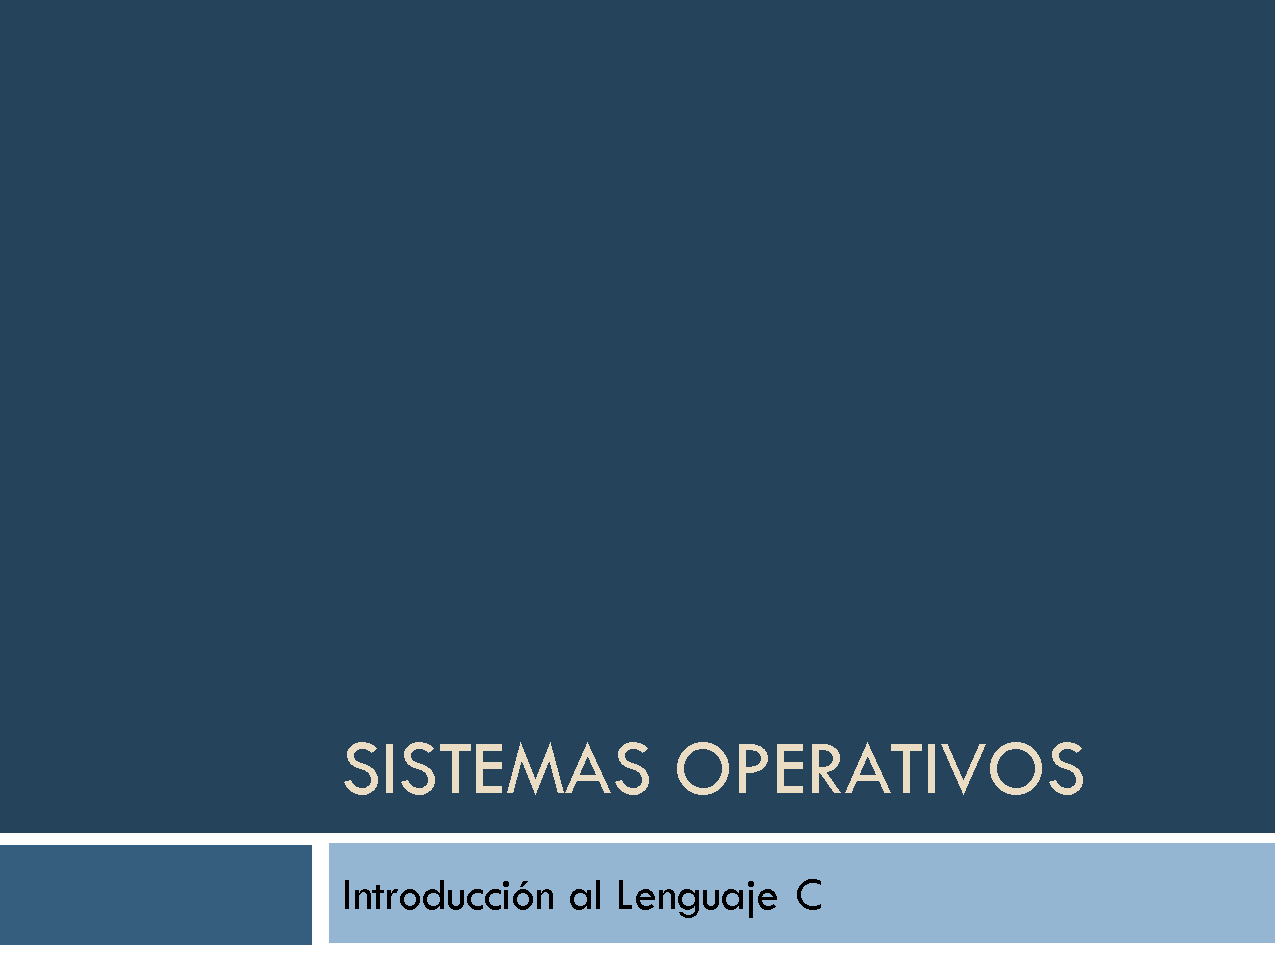
\includepdf[pages=-]{docs/Introduccion_al_Lenguaje_C_(1).pdf}
\includepdf[pages=-]{docs/Presentacion_1.1_Introduccion_y_Conceptos.pdf}
\includepdf[pages=-]{docs/Presentacion_1.2_Servicios_del_SO.pdf}
\includepdf[pages=-]{docs/Presentacion_2.1_Introduccion_a_Gestion_de_Procesos.pdf}
\includepdf[pages=-]{docs/Presentacion_2.2_Planificacion_de_procesos.pdf}
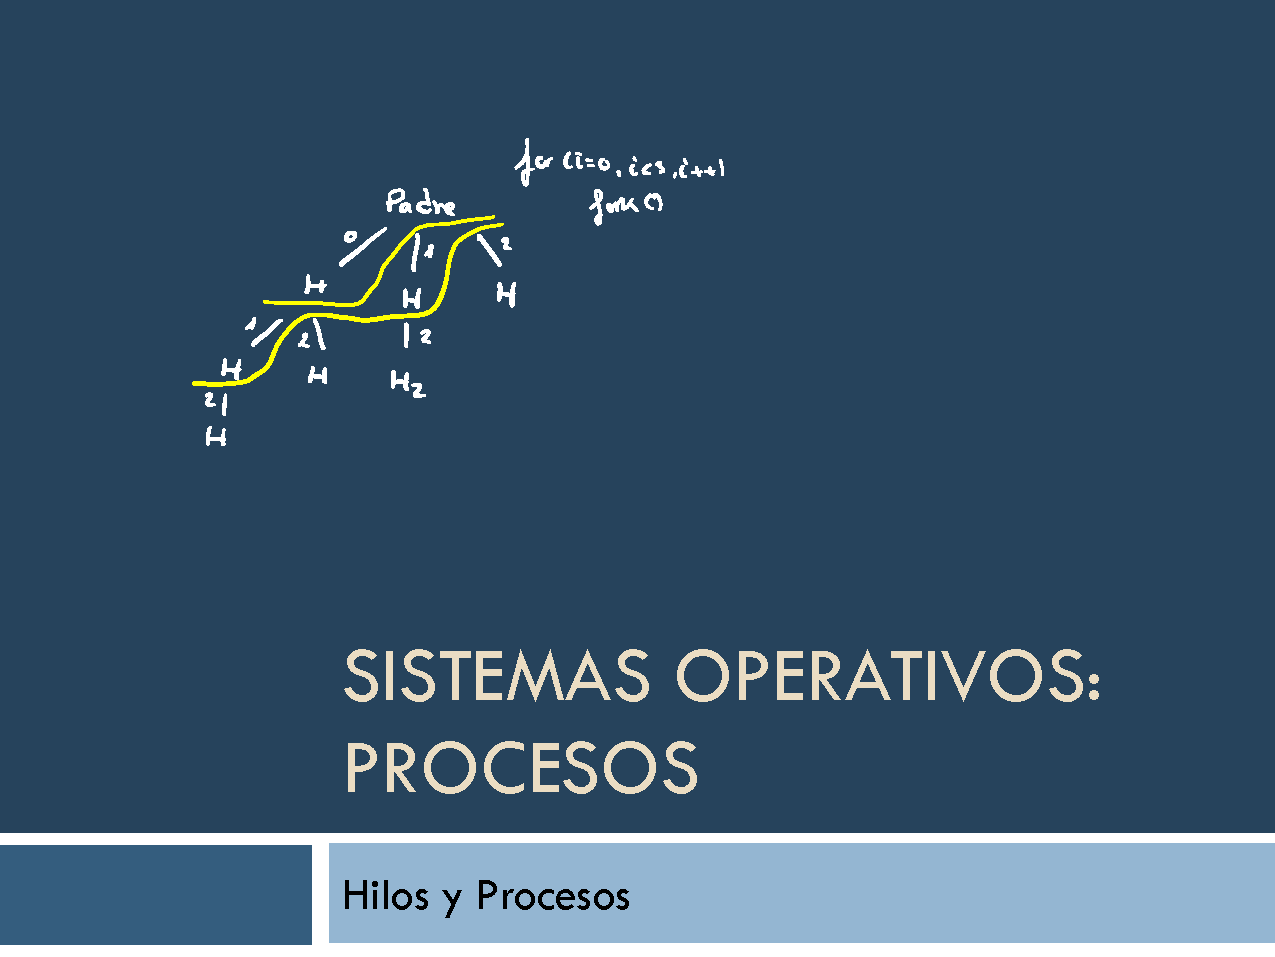
\includepdf[pages=-]{docs/Presentacion_2.3_Hilos_y_Procesos.pdf}
\includepdf[pages=-]{docs/Presentacion_2.4_Senales_excepciones.pdf}
\includepdf[pages=-]{docs/Presentacion_3.1_Introduccion_y_Conceptos.pdf}
\includepdf[pages=-]{docs/Presentacion_3.2_Hilos_y_Mecanismos_Sincronizacion.pdf}
\includepdf[pages=-]{docs/Presentacion_3.3_Desarrollo_Servidores_Concurrentes.pdf}

\includepdf[pages=-]{docs/Presentacion_4.1_Ficheros_.pdf}

\includepdf[pages=-]{docs/Problemas_frecuentes_con_el_lenguaje_C.pdf}
\includepdf[pages=-]{docs/Sesion_2_Problemas_lenguaje_C.pdf}

\includepdf[pages=-]{docs/Sesion_6_Llamadas_al_sistema.pdf}
\includepdf[pages=-]{docs/Sesion_10_Procesos.pdf}
\includepdf[pages=-]{docs/Sesion_12_Tuberias_.pdf}

\includepdf[pages=-]{docs/Sesion_28_Sistema_de_ficheros.pdf}

\part{Ejercicios C}
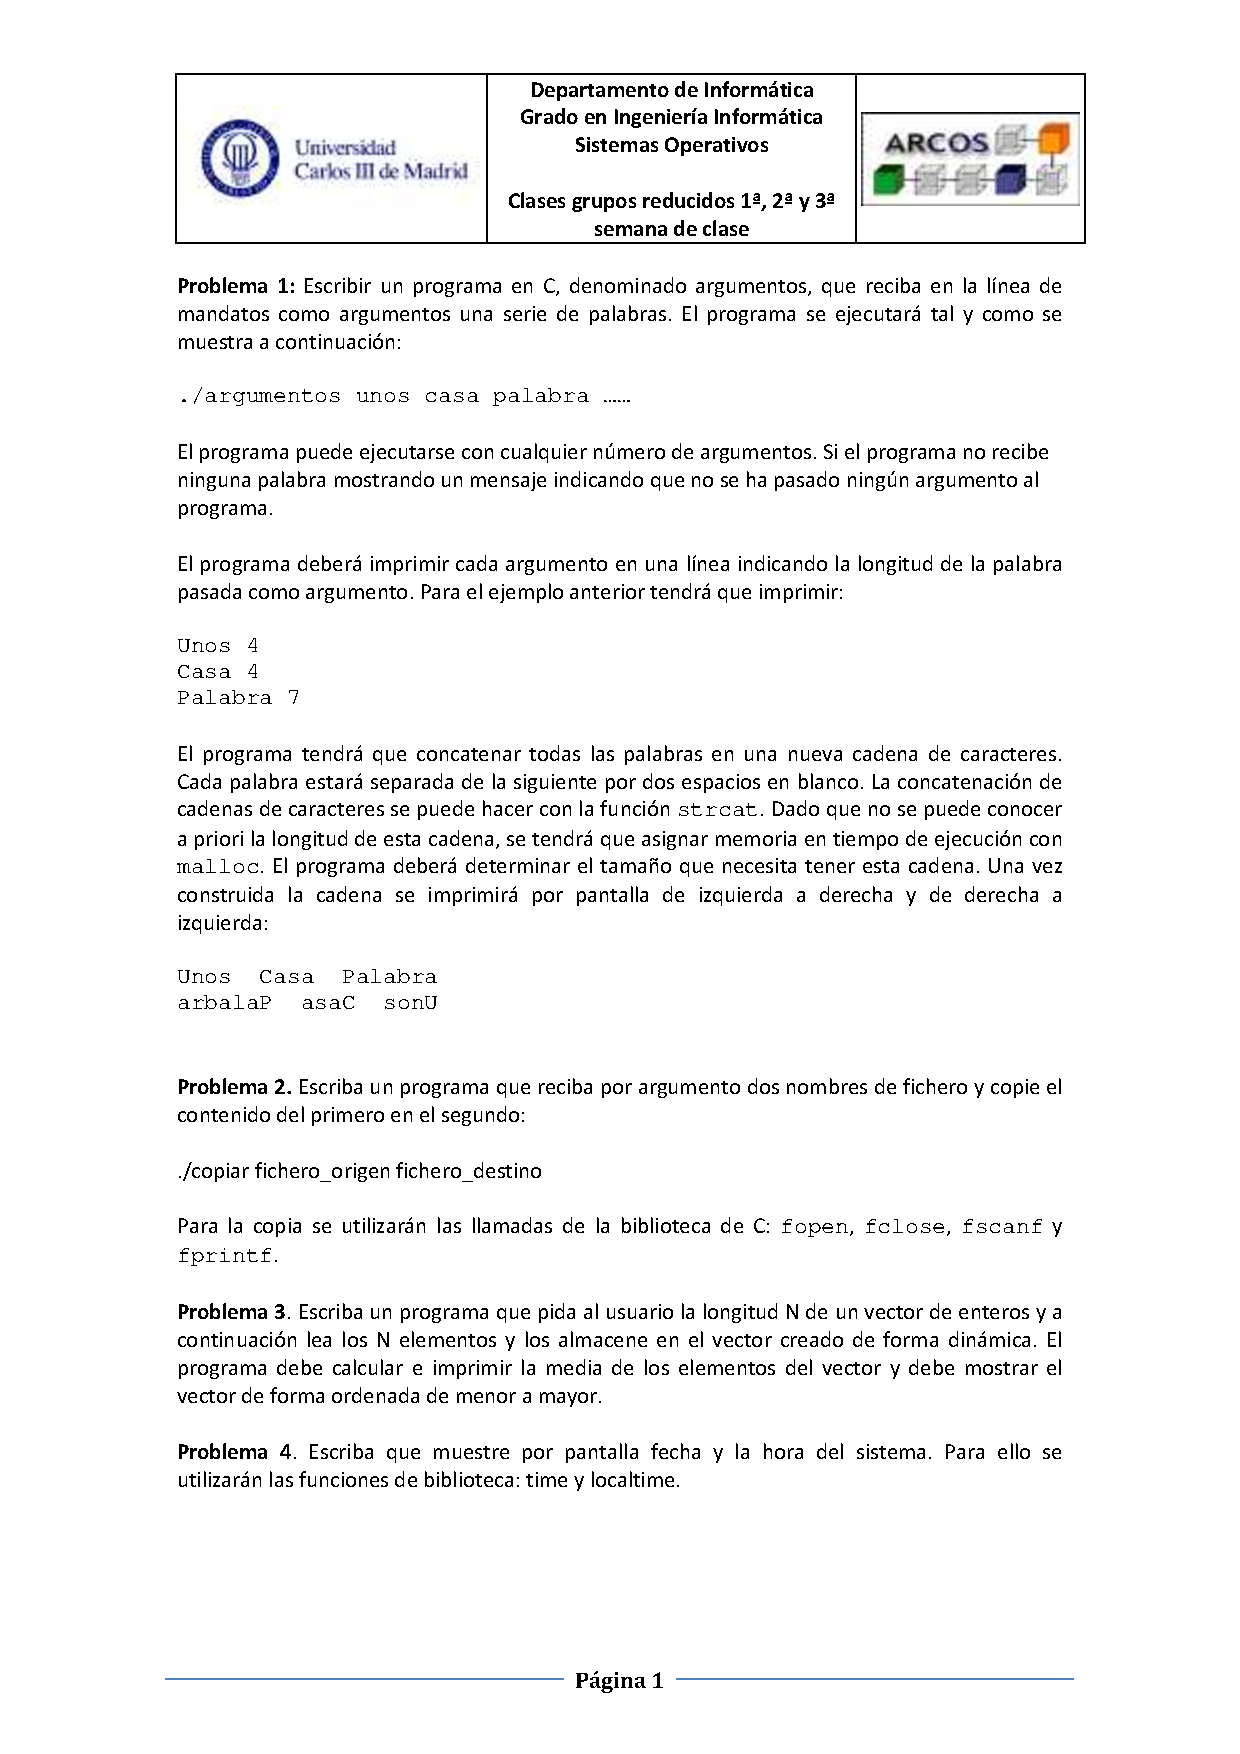
\includepdf[pages=-]{docs/ejercicios-c-2.pdf}
\includepdf[pages=-]{docs/Ejercicios_C.pdf}

\includepdf[pages=-]{docs/03-Problemas_frecuentes_con_el_lenguaje_C.pdf}

\part{Ejercicios teoría y calculo}

\includepdf[pages=-]{docs/01-Problemas_lenguaje_C-01.pdf}
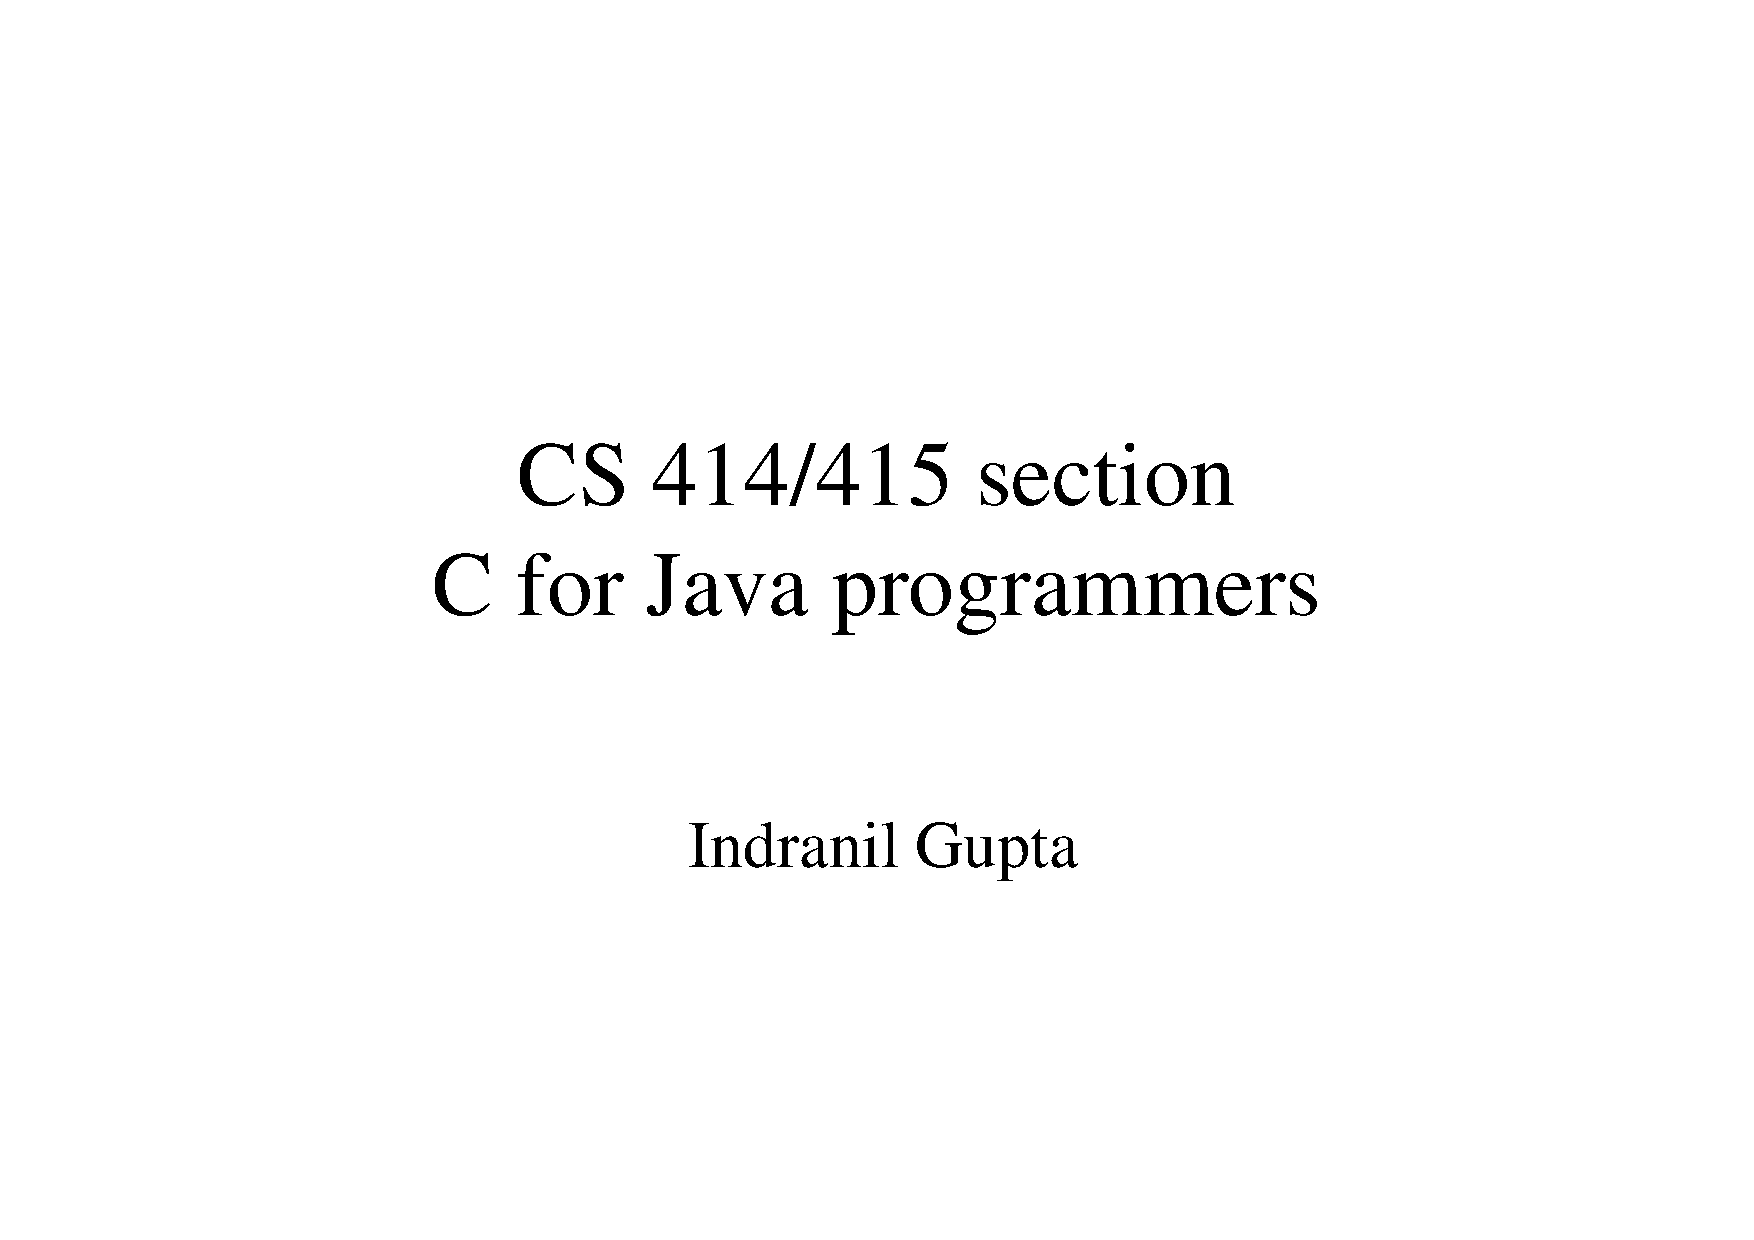
\includepdf[pages=-]{docs/02-c_for_java_programmers.pdf}

\includepdf[pages=-]{docs/04-Llamadas_al_sistema.pdf}
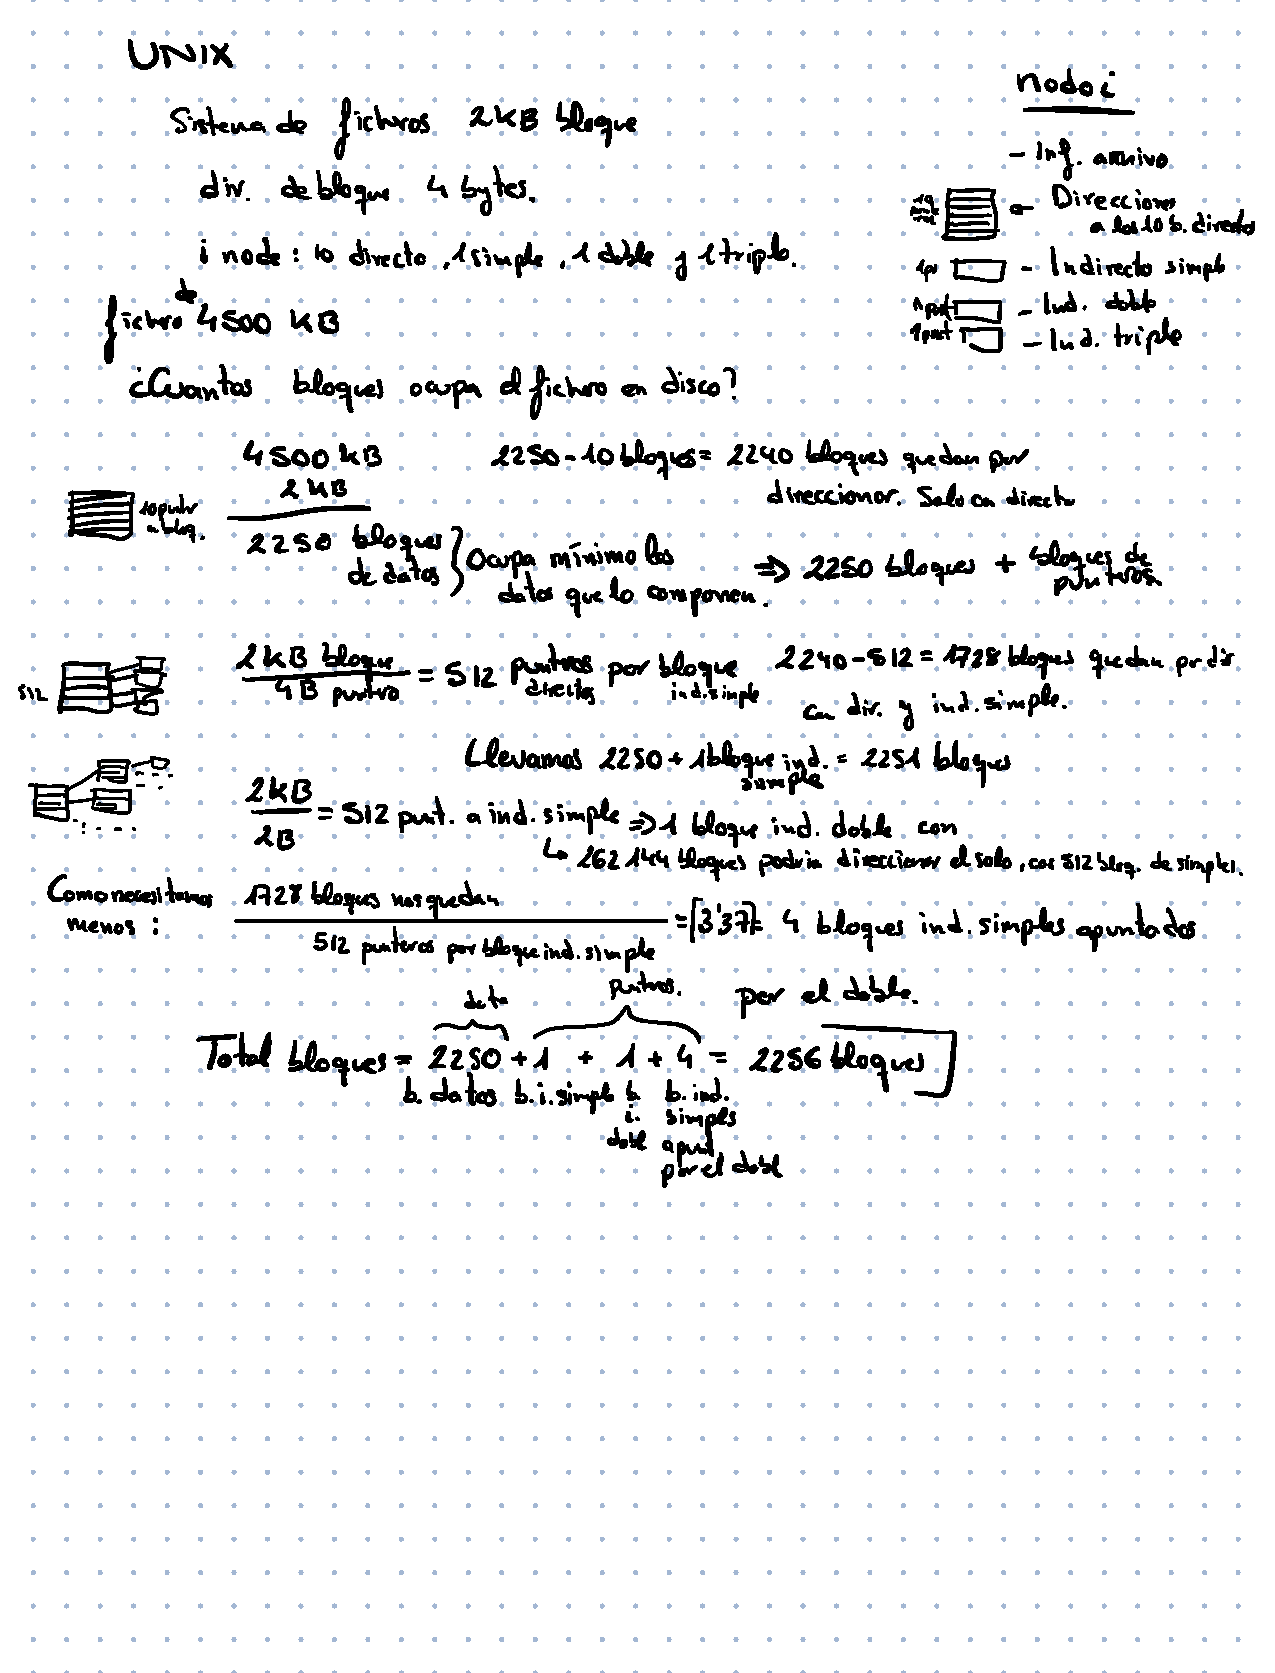
\includepdf[pages=-]{docs/EJ1_T5_L11.pdf}
\includepdf[pages=-]{docs/EJ1_T5_L12.pdf}
\includepdf[pages=-]{docs/EJ1_T5_L13.pdf}
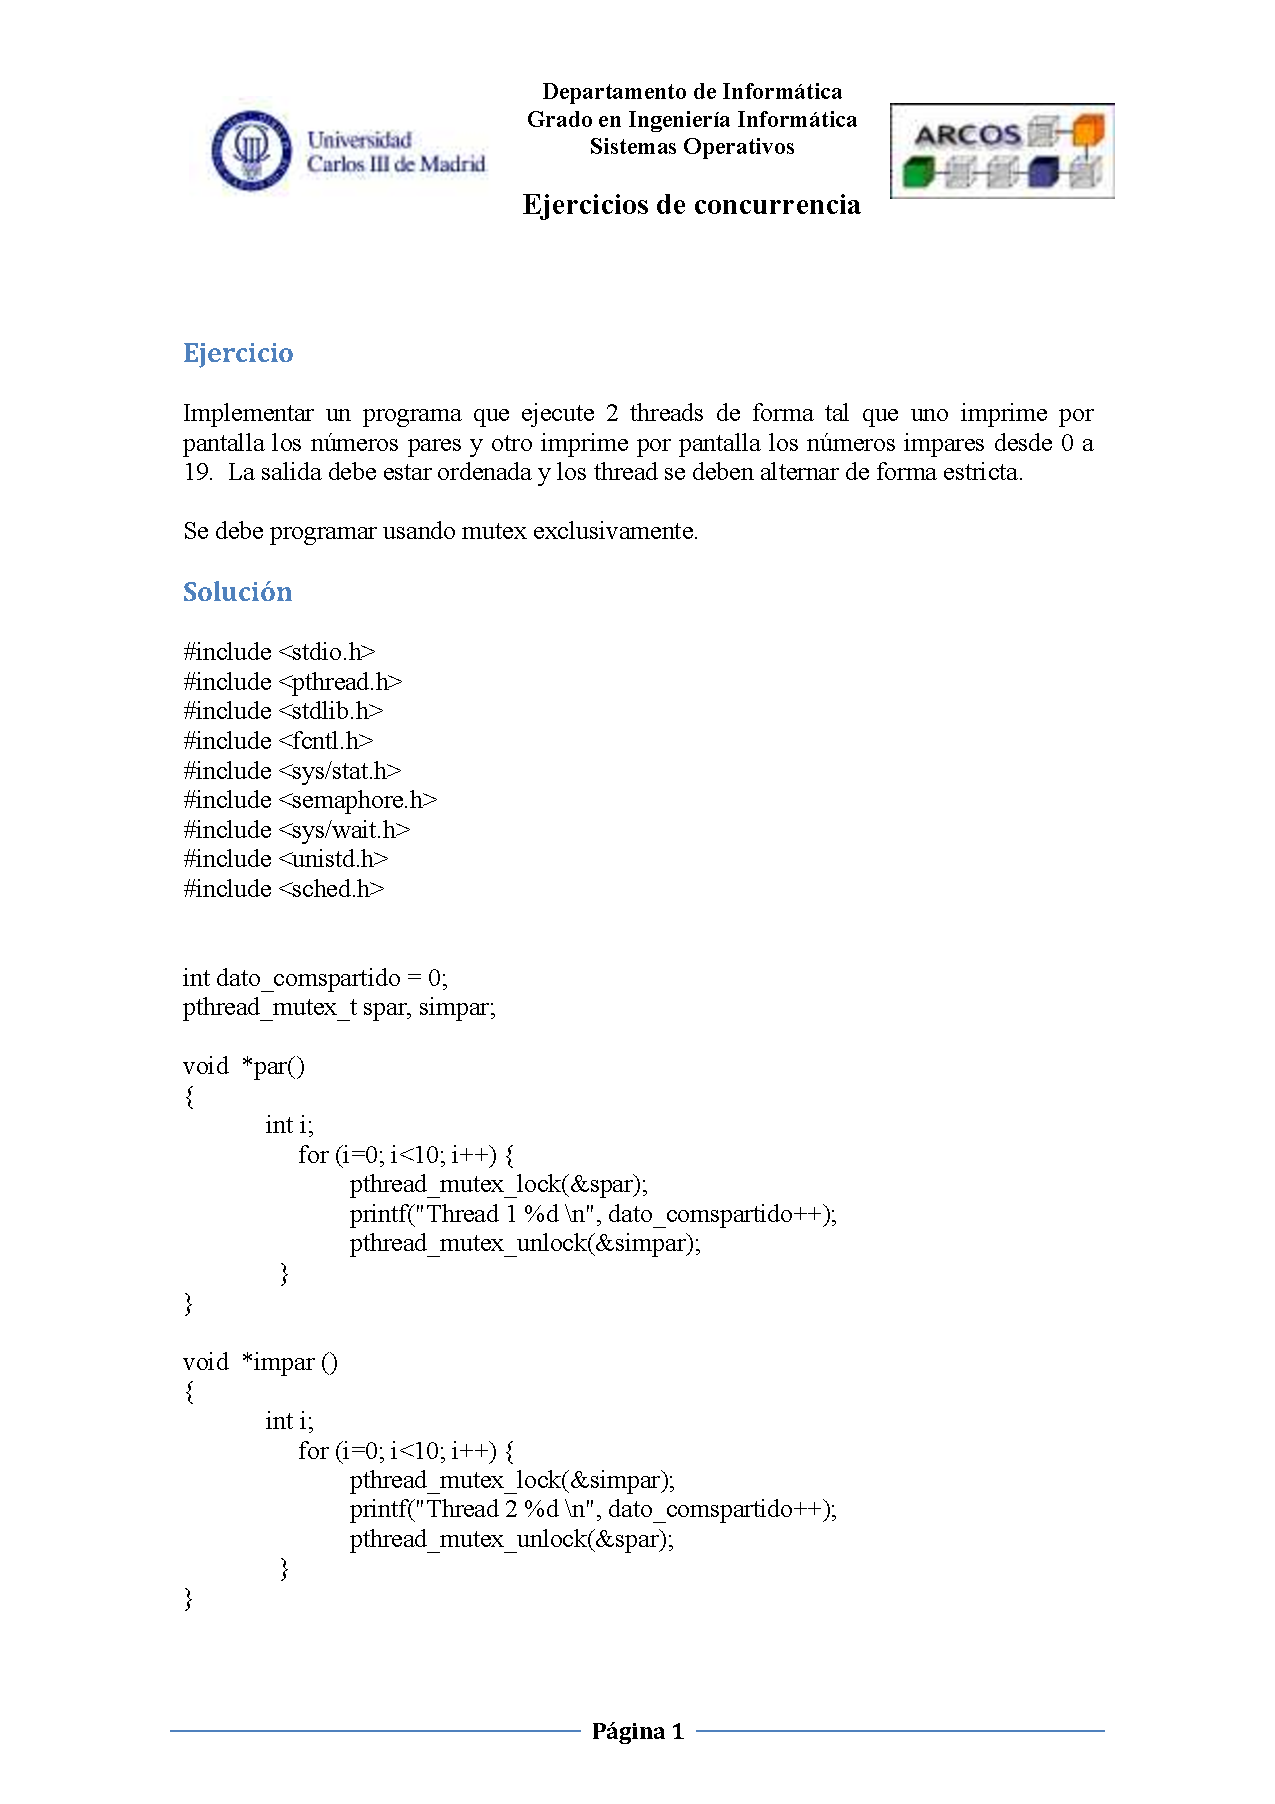
\includepdf[pages=-]{docs/Ejercicios_3-2.pdf}
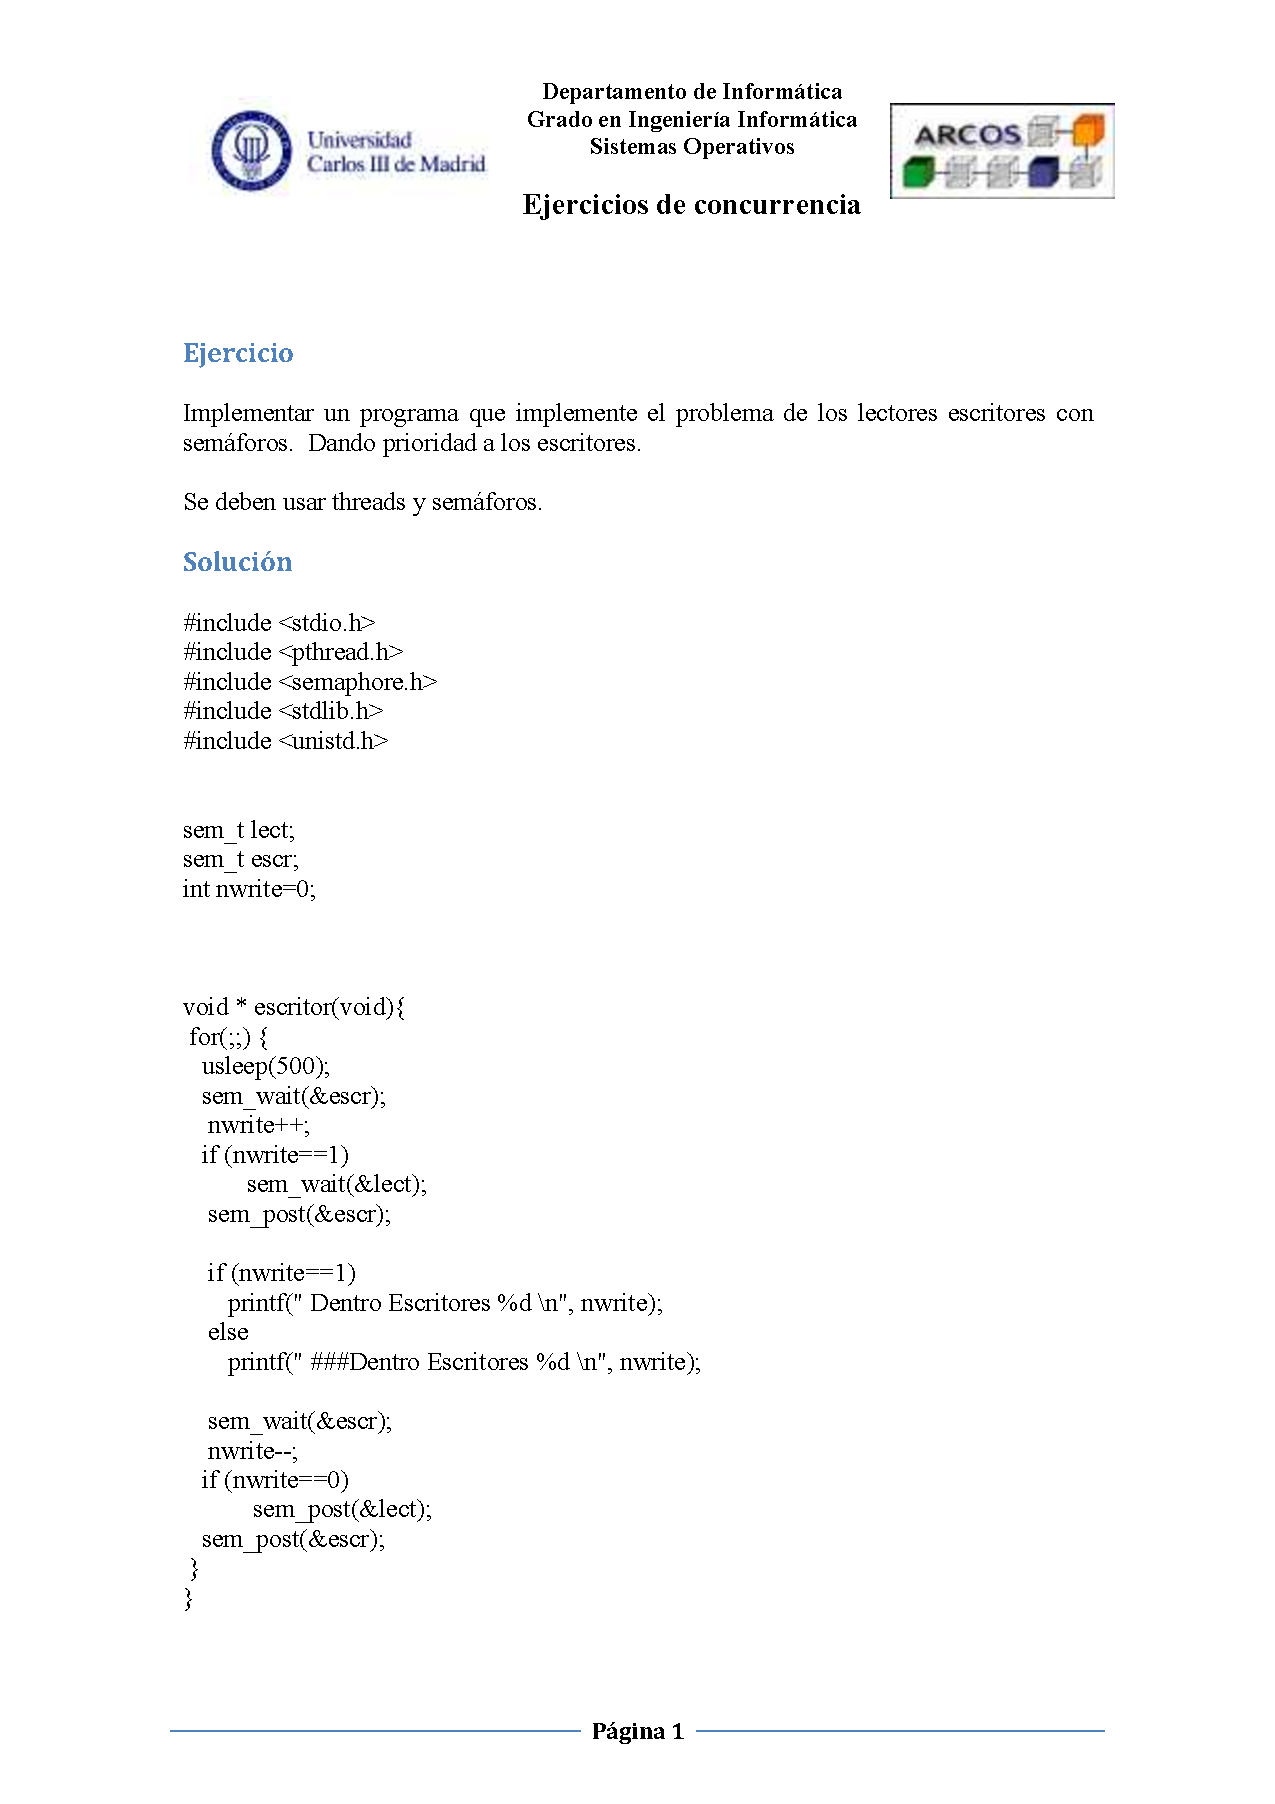
\includepdf[pages=-]{docs/Ejercicios_3-3.pdf}
\includepdf[pages=-]{docs/Ejercicios_3-4_.pdf}
\includepdf[pages=-]{docs/Ejercicios_3-6.pdf}
\includepdf[pages=-]{docs/Ejercicios_C_2.pdf}
\includepdf[pages=-]{docs/Ejercicios_C.pdf}
\includepdf[pages=-]{docs/Ejercicios_Pizarra_SO.pdf}
\includepdf[pages=-]{docs/Ejercicios_T_1.1.pdf}
\includepdf[pages=-]{docs/Ejercicios_T_1.2.pdf}
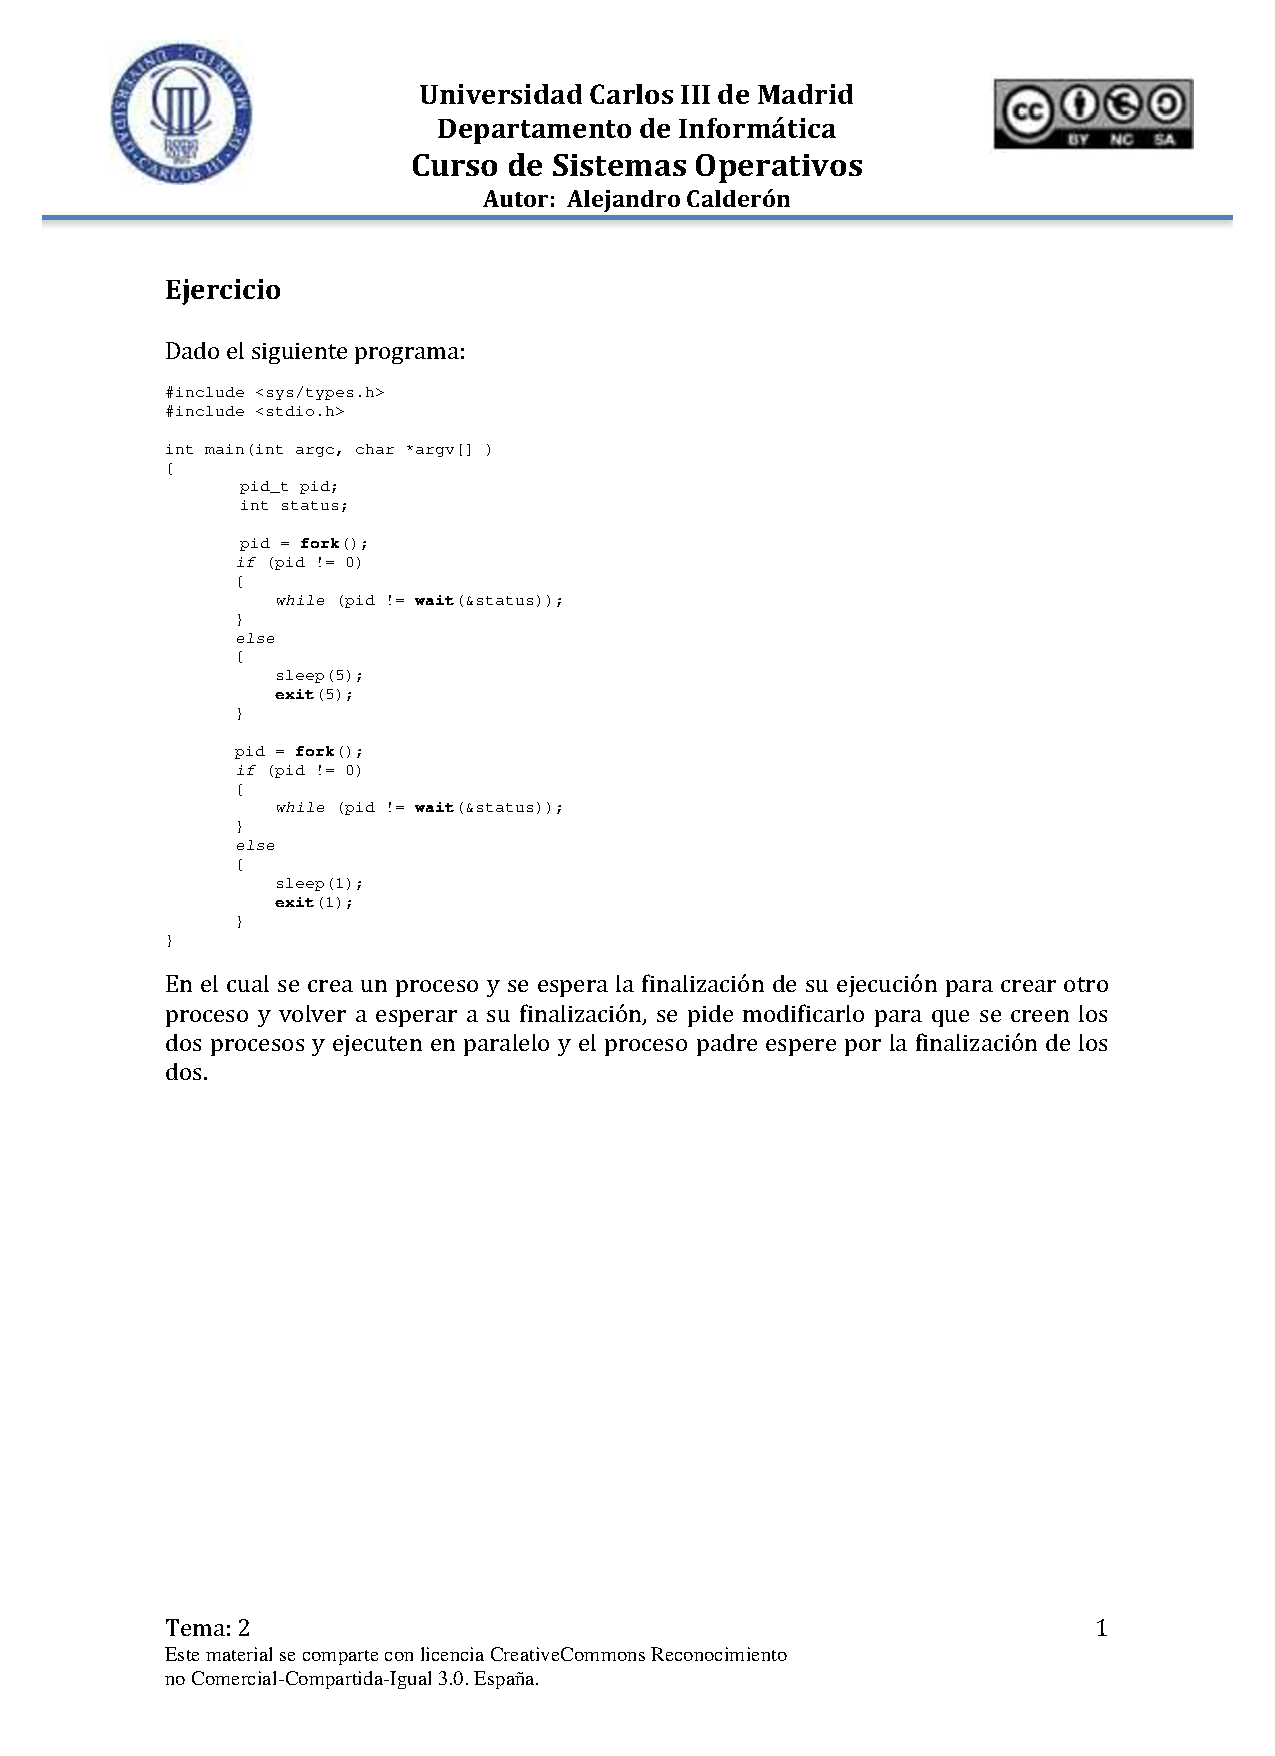
\includepdf[pages=-]{docs/Ejercicios_T_2.1.pdf}
\includepdf[pages=-]{docs/Ejercicios_T_2.2.pdf}
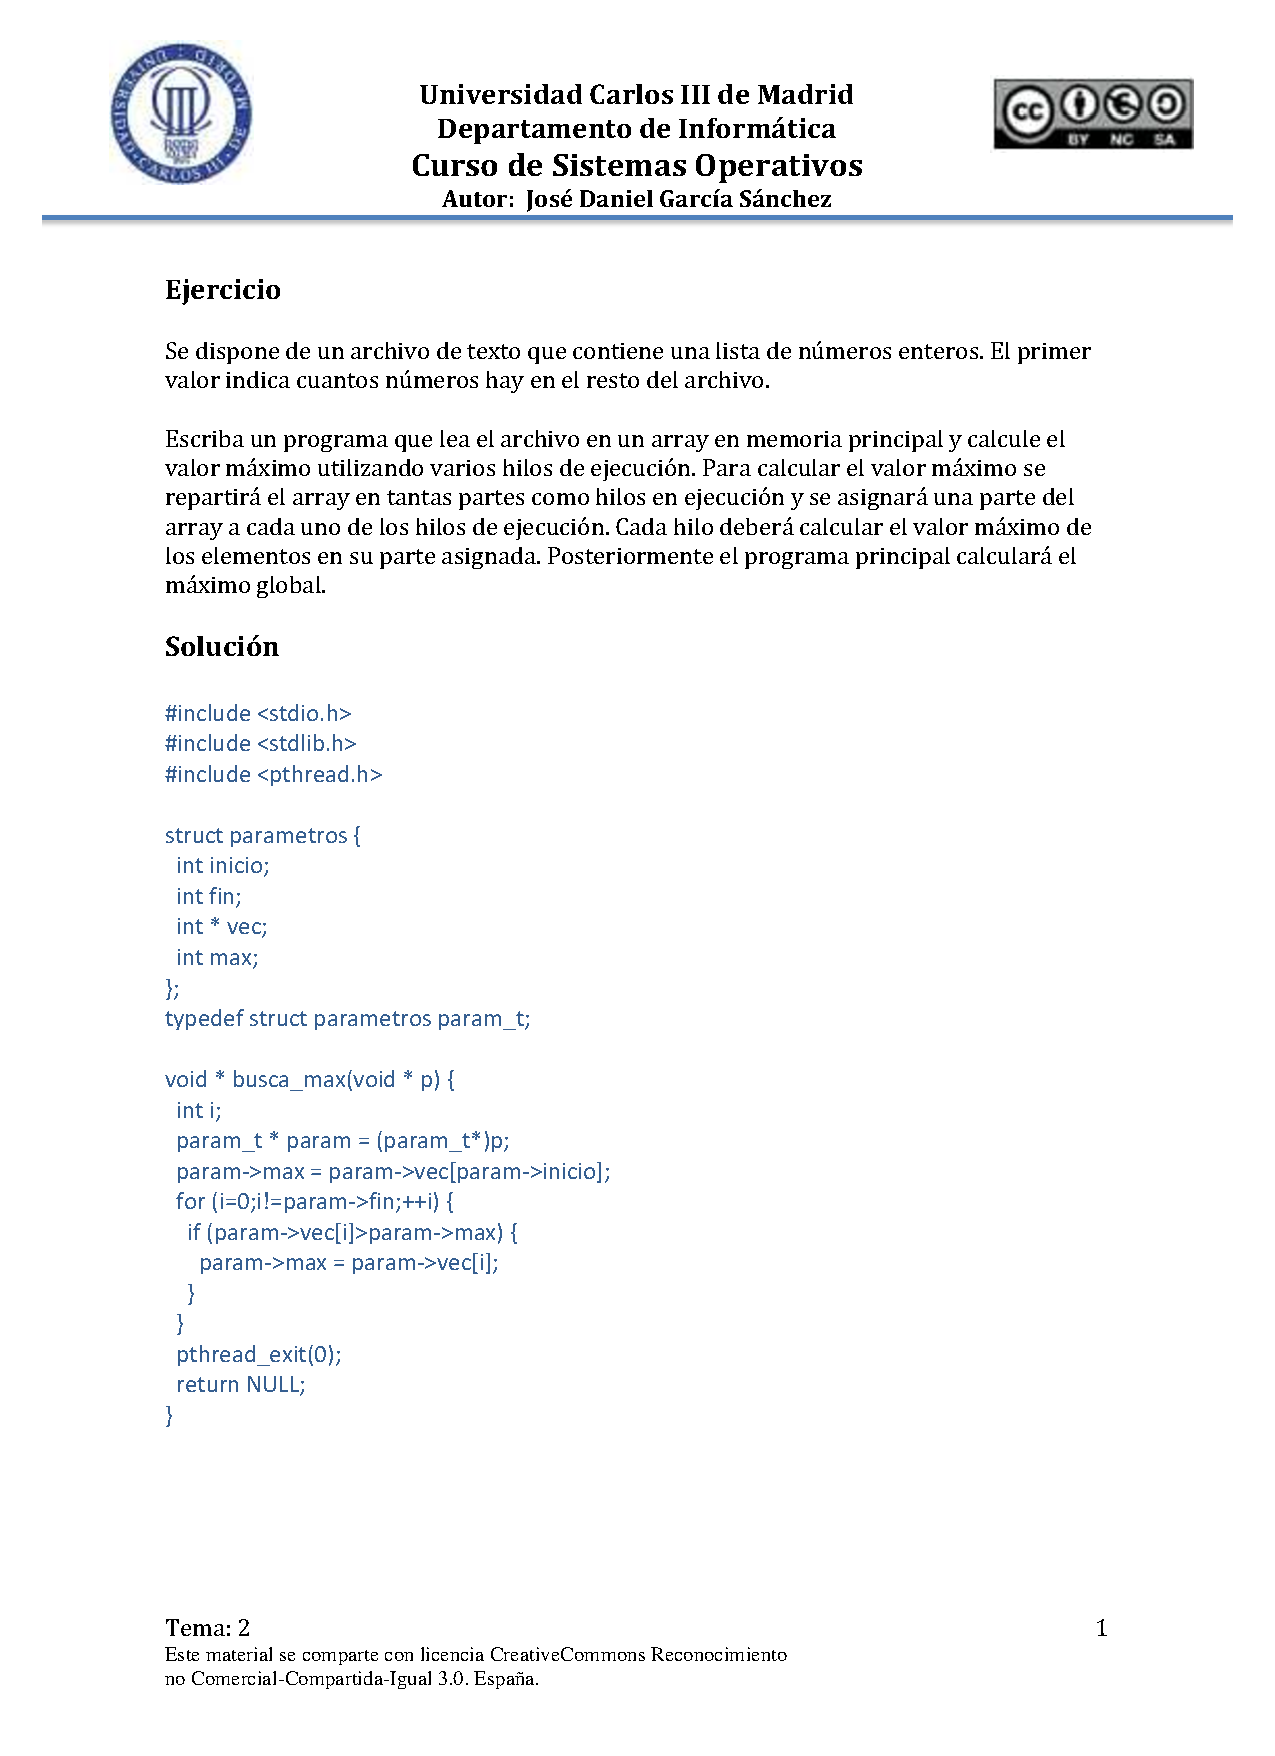
\includepdf[pages=-]{docs/Ejercicios_T_2.3.pdf}
\includepdf[pages=-]{docs/Ejercicios_T_3.0_con_Soluciones_SSOO.pdf}
\includepdf[pages=-]{docs/Ejercicios_T_3.0_SSOO.pdf}
\includepdf[pages=-]{docs/Ejercicios_T_3.1.pdf}
\includepdf[pages=-]{docs/Ejercicios_T_3.2.pdf}
\includepdf[pages=-]{docs/Ejercicios_T_3.3.pdf}
\includepdf[pages=-]{docs/Ejercicios_T_4.1.pdf}
\includepdf[pages=-]{docs/Ejercicios_T_4.2.pdf}
\includepdf[pages=-]{docs/Ejercicios_T_4.3.pdf}
\includepdf[pages=-]{docs/ejercicios-18-03.pdf}
\includepdf[pages=-]{docs/Nota_13_may_2020_9_36_25.pdf}
\includepdf[pages=-]{docs/Nota_20_may_2020_1_47_58.pdf}
\includepdf[pages=-]{docs/Nota_28_abr_2020_12_41_04.pdf}
\includepdf[pages=-]{docs/pipes-sincronizacion.pdf}
\includepdf[pages=-]{docs/Practica_1._Llamadas_al_sistema.pdf}
\includepdf[pages=-]{docs/Practica_2._MiniShell.pdf}
\includepdf[pages=-]{docs/sem-nombre-par-impar.pdf}

\part{Test}
\includepdf[pages=-]{docs/SSOO_AutoTest_1.pdf}
\includepdf[pages=-]{docs/SSOO_Autotest_2.pdf}
\includepdf[pages=-]{docs/SSOO_Autotest_3.pdf}
\includepdf[pages=-]{docs/SSOO_Autotest_soluciones.pdf}

\part{Exámenes}
\includepdf[pages=-]{docs/2009-grado-ssoo-examen-junio-extraordinario-colme-v2.pdf}
\includepdf[pages=-]{docs/2009-ssoo-ordinario-1p.pdf}
\includepdf[pages=-]{docs/2009-ssoo-ordinario-2p-sol.pdf}
\includepdf[pages=-]{docs/2009-ssoo-ordinario-2p.pdf}
\includepdf[pages=-]{docs/2009-ssoo-parcial-sol.pdf}
\includepdf[pages=-]{docs/2009-ssoo-parcial.pdf}
\includepdf[pages=-]{docs/2009grado-ssoo-examen-junio-extraordinario-colme-test.pdf}
\includepdf[pages=-]{docs/2010-ssoo-colme-parcial-sol.pdf}
\includepdf[pages=-]{docs/2010-ssoo-colme-parcial.pdf}
\includepdf[pages=-]{docs/2010-ssoo-ordinario-sol.pdf}
\includepdf[pages=-]{docs/2010-ssoo-parcial-sol-b.pdf}
\includepdf[pages=-]{docs/2010-ssoo-parcial-sol.pdf}
\includepdf[pages=-]{docs/2011-ssoo-extrordinario-sol.pdf}
\includepdf[pages=-]{docs/2013-Parcial-G83-A-Sol.pdf}
\includepdf[pages=-]{docs/2013-Parcial-G83-B-Sol.pdf}
\includepdf[pages=-]{docs/2013-Parcial-Jorge-Sol.pdf}
\includepdf[pages=-]{docs/ejercicios_procesos_senyales_y_planificacion.pdf}
\includepdf[pages=-]{docs/Examen_1_SOL.pdf}
\includepdf[pages=-]{docs/Examen_1P_enero-2010_SOL.pdf}
\includepdf[pages=-]{docs/Examen_1P_enero-2010.pdf}
\includepdf[pages=-]{docs/Examen_2_SOL.pdf}
\includepdf[pages=-]{docs/Examen_2P_enero-2010.pdf}
\includepdf[pages=-]{docs/Examen_3_SOL.pdf}
\includepdf[pages=-]{docs/Examen_extraordinario_junio-2010.pdf}
\includepdf[pages=-]{docs/Examen_extraordinario_ssoo_junio-2010_Solucion_(2).pdf}
\includepdf[pages=-]{docs/Examen_extraordinario_ssoo_junio-2010.pdf}
\includepdf[pages=-]{docs/examen-extraordinario-2014-2015-sol.pdf}
\includepdf[pages=-]{docs/examen-ordinario-2014-2015-solucion.pdf}
\includepdf[pages=-]{docs/examEnero2012ssooParte1-publicar.pdf}
\includepdf[pages=-]{docs/ExamExtraordSSOOjun2010v240610.pdf}
\includepdf[pages=-]{docs/ExSSOOen2013.pdf}
\includepdf[pages=-]{docs/ExSSOOjun2010_SOL.pdf}
\includepdf[pages=-]{docs/ExSSOOJun2011-definitivo.pdf}
\includepdf[pages=-]{docs/ExSSOOJun2011v3-sol.pdf}
\includepdf[pages=-]{docs/ExSSOOsep2010_SOLv030910_(2).pdf}
\includepdf[pages=-]{docs/ExSSOOsep2010_SOLv030910.pdf}
\includepdf[pages=-]{docs/grado-ssoo-examen-junio-extraordinario-colme-v2.pdf}
\includepdf[pages=-]{docs/II-SSOO-2006-junio-colmenarejo-parcial01-G81.pdf}
\includepdf[pages=-]{docs/II-SSOO-2007-junio-1pE-sol.pdf}
\includepdf[pages=-]{docs/II-SSOO-2007-junio-2pE-sol.pdf}
\includepdf[pages=-]{docs/II-SSOO-2007-sept-sol.pdf}
\includepdf[pages=-]{docs/itig-ssoo-2008-junio-sol.pdf}
\includepdf[pages=-]{docs/itig-ssoo-2008-sept-sol.pdf}
\includepdf[pages=-]{docs/parcial_(2).pdf}
\includepdf[pages=-]{docs/parcial_SSOO_sol_colme50-1.pdf}
\includepdf[pages=-]{docs/parcial-solucion_(2).pdf}
\includepdf[pages=-]{docs/parcial-solucion.pdf}
\includepdf[pages=-]{docs/parcial.pdf}
\includepdf[pages=-]{docs/Primer_Parcial_SSOO_2010-2011-grs-81-82-83.pdf}
\includepdf[pages=-]{docs/Primer_Parcial_SSOO_2010-2011-grs-84-85-solucion.pdf}
\includepdf[pages=-]{docs/Primer_Parcial_SSOO_2010-2011-grs-84-85.pdf}
\includepdf[pages=-]{docs/primer-parcial-8182-octubre-2009.pdf}
\includepdf[pages=-]{docs/primer-parcial-8384-octubre-2009.pdf}
\includepdf[pages=-]{docs/primer-parcial-colme-2008-2009.pdf}
\includepdf[pages=-]{docs/solexjun2006.pdf}
\includepdf[pages=-]{docs/solexjun2007.pdf}
\includepdf[pages=-]{docs/solexsep2007.pdf}
\includepdf[pages=-]{docs/solexsept2006.pdf}
\includepdf[pages=-]{docs/SSOO_extraordinario_2014_Mod1-sol.pdf}
\includepdf[pages=-]{docs/SSOO_extraordinario_jun_2013_problemas-solucion.pdf}
\includepdf[pages=-]{docs/SSOO_extraordinario_jun_2013_v1_-_sol.pdf}
\includepdf[pages=-]{docs/SSOO_g_ii_primer_parcial_8485_octubre-2010_solucion.pdf}
\includepdf[pages=-]{docs/SSOO_g_ii_primer_parcial_Colmenarejo_octubre-2010_solucion.pdf}
\includepdf[pages=-]{docs/SSOO_ordinaria_2014_solucion.pdf}
\includepdf[pages=-]{docs/SSOO_ordinario_jun_2013_v1-sol.pdf}
\includepdf[pages=-]{docs/SSOO_parcial_2014_g8182_solucion.pdf}
\includepdf[pages=-]{docs/SSOO_parcial_2014_Mod6_sol.pdf}
\includepdf[pages=-]{docs/SSOO_parcial_2015_g8182TipoASolucionv120315b.pdf}
\includepdf[pages=-]{docs/SSOO_primer_parcial_81_2013.pdf}
\includepdf[pages=-]{docs/ssoo-final-test-modelo-C_sol.pdf}
\includepdf[pages=-]{docs/ssoo-ordinario-febreo-2011.pdf}
\includepdf[pages=-]{docs/ssoo-ssh-actividad-2013.pdf}

\part{Practica 1. Llamadas al sistema}
\includepdf[pages=-]{docs/ssoo_p1_100405951_100405834.pdf}
\includepdf[pages=-]{docs/notas_p1_ssoo_81.pdf}
\includepdf[pages=-]{docs/p1_llamadas_al_sistema_19-20.pdf}

\part{Practica 2. MiniShell}
\includepdf[pages=-]{docs/p2_minishell_enunciado_19-20.pdf}
\includepdf[pages=-]{docs/p2_minishell_transparencias_19-20.pdf}
\includepdf[pages=-]{docs/tuberias.pdf}
\includepdf[pages=-]{docs/ssoo_p2_100405951_100405834.pdf}

\part{Practica 3. Multi-hilo}
\includepdf[pages=-]{docs/ssoo_p3_multithread_19-20.pdf}
\includepdf[pages=-]{docs/ssoo_p3_100405951_100405834.pdf}

\part{Recursos}
\includepdf[pages=-]{docs/errores-frecuentes-C.pdf}
\includepdf[pages=-]{docs/Guia_C.pdf}
\includepdf[pages=-]{docs/Lenguaje-C.pdf}
\includepdf[pages=-]{docs/Principales_comandos_del_editor_vi.pdf}

\end{document}